% !TeX program = xelatex
\documentclass[UTF8,11pt,openany,fontset=none]{ctexbook}
\defaultCJKfontfeatures{}
% Prefer TrueType CJK fonts: xdvipdfmx embeds explicit ToUnicode maps for them.
% This avoids relying on a PDF viewer's external Adobe CJK character maps.
\IfFontExistsTF{SimSun}{%
  \setCJKmainfont[BoldFont=SimHei,ItalicFont=KaiTi,BoldItalicFont=KaiTi]{SimSun}
  \setCJKsansfont[BoldFont=Microsoft YaHei Bold]{Microsoft YaHei}
  \setCJKmonofont{SimSun}
}{%
  \setCJKmainfont[BoldFont=FandolSong-Bold,ItalicFont=FandolKai-Regular]{FandolSong-Regular}
  \setCJKsansfont[BoldFont=FandolHei-Bold]{FandolHei-Regular}
  \setCJKmonofont{FandolFang-Regular}
}
\usepackage[a4paper,inner=24mm,outer=21mm,top=24mm,bottom=24mm,headheight=16pt]{geometry}
\usepackage{lmodern}
\usepackage{amsmath,amssymb,mathtools,bm,mathrsfs}
\usepackage[dvipsnames]{xcolor}
\usepackage[most]{tcolorbox}
\usepackage{tikz,pgfplots,booktabs,array,longtable,tabularx,enumitem,fancyhdr,graphicx}
\usepackage{titletoc,multicol,needspace}
\usepackage{fvextra}
\usepackage{hyperref,cleveref}
\fvset{fontsize=\footnotesize,breaklines=true,breakanywhere=false,numbers=left,
  breaksymbolleft=\textcolor{Rust}{$\hookrightarrow$},
  numbersep=5pt,xleftmargin=5mm,baselinestretch=1.05,
  frame=leftline,rulecolor=\color{Teal!45}}
\pgfplotsset{compat=1.18}
\definecolor{Ink}{HTML}{19364A}
\definecolor{Teal}{HTML}{227C81}
\definecolor{Gold}{HTML}{A87830}
\definecolor{Rust}{HTML}{9B483A}
\definecolor{CoverTeal}{HTML}{20ADAA}
\definecolor{CoverGold}{HTML}{DDBD35}
\hypersetup{colorlinks=true,linkcolor=Teal,urlcolor=Teal,citecolor=Teal,
  bookmarksnumbered=true,pdftitle={Python 网络爬虫：从请求到数据},
  pdfauthor={雪落长安无声},pdfsubject={Python 网络爬虫学习笔记}}
\ctexset{chapter={format=\Huge\bfseries\color{Ink},beforeskip=10pt,afterskip=22pt},section={format=\Large\bfseries\color{Teal}},subsection={format=\large\bfseries\color{Ink}}}
\setcounter{tocdepth}{2}
\setcounter{secnumdepth}{2}
% openany also applies when switching from front matter to main matter.
\let\cleardoublepage\clearpage
\pagestyle{fancy}\fancyhf{}
\fancyhead[LE,RO]{\small\color{Ink}\thepage}
\fancyhead[LO]{\small\nouppercase{\leftmark}}
\fancyhead[RE]{\small Python 网络爬虫：从请求到数据}
\renewcommand{\headrulewidth}{0.4pt}
\fancypagestyle{plain}{\fancyhf{}\fancyfoot[C]{\small\thepage}\renewcommand{\headrulewidth}{0pt}}
\tcbset{enhanced,breakable,boxrule=0.45pt,arc=1mm,left=2mm,right=2mm,top=1.2mm,bottom=1.2mm,before skip=8pt,after skip=8pt,fonttitle=\bfseries,colback=white,colframe=Teal}
\newcounter{statement}[chapter]\renewcommand{\thestatement}{\thechapter.\arabic{statement}}
\newenvironment{definition}[1]{\refstepcounter{statement}\begin{tcolorbox}[title={定义\thestatement\quad #1},colback=Teal!3]}{\end{tcolorbox}}
\newenvironment{theorem}[1]{\refstepcounter{statement}\begin{tcolorbox}[title={定理\thestatement\quad #1},colback=Ink!3,colframe=Ink]}{\end{tcolorbox}}
\newenvironment{lemma}[1]{\refstepcounter{statement}\begin{tcolorbox}[title={引理\thestatement\quad #1}]}{\end{tcolorbox}}
\newenvironment{corollary}[1]{\refstepcounter{statement}\begin{tcolorbox}[title={推论\thestatement\quad #1}]}{\end{tcolorbox}}
\newenvironment{proof}{\begin{tcolorbox}[title=原理与推导,colframe=Ink,colbacktitle=Ink,coltitle=white,colback=Ink!2]}{\end{tcolorbox}}
\newenvironment{method}[1]{\begin{tcolorbox}[title={方法卡\quad #1},colframe=Teal,colback=Teal!3]}{\end{tcolorbox}}
\newenvironment{warning}{\begin{tcolorbox}[title=常见错误与边界,colframe=Rust,colback=Rust!3]}{\end{tcolorbox}}
\newenvironment{examtip}{\begin{tcolorbox}[title=实践提示,colframe=Gold,colback=Gold!4]}{\end{tcolorbox}}
\newenvironment{extension}{\begin{tcolorbox}[title=进阶实践,colframe=Gold,colback=Gold!4]}{\end{tcolorbox}}
\newcounter{example}[chapter]\renewcommand{\theexample}{\thechapter.\arabic{example}}
\newenvironment{example}[2]{\refstepcounter{example}\begin{tcolorbox}[title={例\theexample\quad #1\quad #2},title after break={例\theexample\quad #1（续）},colframe=Ink]}{\end{tcolorbox}}
\newcounter{exercise}[chapter]\renewcommand{\theexercise}{\thechapter.\arabic{exercise}}
\newcommand{\dd}{\mathop{}\!\mathrm{d}}
\newcommand{\e}{\mathrm{e}}
\newcommand{\R}{\mathbb{R}}
\newcommand{\grad}{\nabla}
\DeclareMathOperator{\diver}{div}
\DeclareMathOperator{\rot}{rot}
\DeclareMathOperator{\sgn}{sgn}
\newcommand{\abs}[1]{\left|#1\right|}
\setlength{\parindent}{2em}\setlength{\parskip}{3pt}
\setlist{nosep,topsep=4pt,leftmargin=2em}
\renewcommand{\arraystretch}{1.25}
\emergencystretch=2em
\raggedbottom

% Printed contents follows the compact two-column chapter/section layout.
% Subsections remain available through the PDF bookmarks.
\definecolor{ContentsBlue}{HTML}{3578C4}
\hypersetup{bookmarksdepth=2}
\ctexset{chapter/tocline={\CTEXifname{\protect\numberline{\thechapter}}{}#2}}
\titlecontents{chapter}[1.7em]
  {\Needspace{3\baselineskip}\addvspace{6pt}\bfseries\color{black}}
  {\contentslabel{1.7em}}{}
  {\hfill\contentspage}[\addvspace{1pt}]
\titlecontents{section}[3.4em]
  {\color{black}}
  {\contentslabel{2.6em}}{}
  {\hspace{.5em}\titlerule*[.7pc]{.}\contentspage}
\contentsmargin{2.5em}
\makeatletter
\newcommand{\booktableofcontents}{%
  \clearpage
  \begingroup
  \pagestyle{plain}\markboth{目录}{目录}%
  \hypersetup{linkcolor=black}%
  \phantomsection\pdfbookmark[0]{目录}{book.contents}%
  \setlength{\parskip}{0pt}%
  \setlength{\columnsep}{8mm}\setlength{\columnseprule}{0pt}%
  \setlength{\multicolsep}{0pt}%
  \vspace*{-2mm}%
  \begin{center}{\fontsize{20}{26}\selectfont\bfseries\color{ContentsBlue}目录}\end{center}%
  \vspace{5mm}%
  \c@tocdepth=1\relax
  \begin{multicols}{2}%
    \fontsize{9.5}{14}\selectfont\raggedcolumns
    \@starttoc{toc}%
  \end{multicols}%
  \clearpage
  \endgroup
}
\makeatother

\begin{document}
\frontmatter
\begin{titlepage}\thispagestyle{empty}
\begin{tikzpicture}[remember picture,overlay]
  \begin{scope}
    \clip(current page.north west) rectangle ([yshift=-76mm]current page.north east);
    \node[inner sep=0pt,anchor=center] at ([yshift=-38mm]current page.north)
      {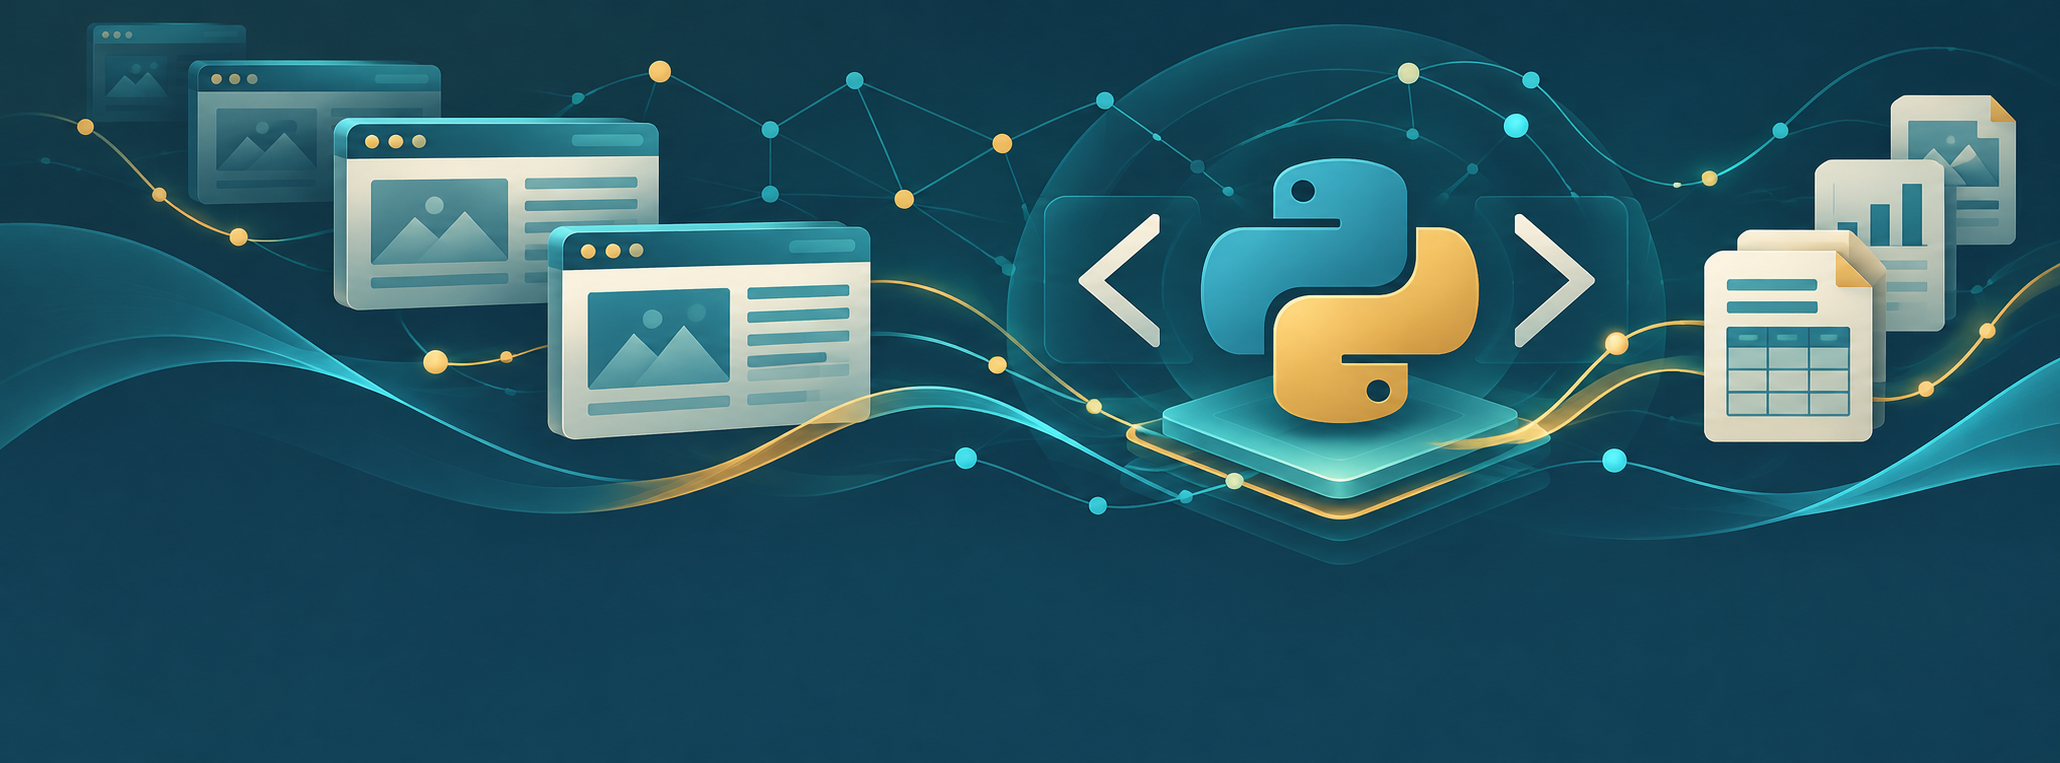
\includegraphics[width=\paperwidth]{assets/cover_network.png}};
  \end{scope}
  \fill[CoverTeal]([yshift=-76mm]current page.north west)
    rectangle ([yshift=-88mm]current page.north east);
  \node[anchor=north west,inner sep=0pt,text=black] at ([xshift=18mm,yshift=-109mm]current page.north west)
    {\fontsize{32}{40}\selectfont\sffamily\bfseries Python 网络爬虫};
  \node[anchor=north west,inner sep=0pt,text=black] at ([xshift=19mm,yshift=-129mm]current page.north west)
    {\fontsize{23}{30}\selectfont\sffamily\bfseries 从请求到数据};
  \node[anchor=north west,inner sep=0pt,text=Ink] at ([xshift=20mm,yshift=-151mm]current page.north west)
    {\fontsize{18}{23}\selectfont\bfseries Python Web Scraping Notes};
  \node[anchor=north west,inner sep=0pt,text=black!58,align=left] at ([xshift=23mm,yshift=-177mm]current page.north west)
    {\fontsize{12}{24}\selectfont
      \begin{tabular}{@{}l@{\;}l@{}}
      作者：&雪落长安无声\\
      日期：&2026.11.05\\
      版本：&2026 年修订
      \end{tabular}};
  \begin{scope}[shift={([xshift=-39mm,yshift=-207mm]current page.north east)}]
    \foreach \x/\y in {-1.2/0.4,-0.5/1.1,0.5/1.4,1.3/0.5,0.7/-0.5,-0.6/-0.8}{
      \draw[CoverGold!65,line width=.5pt] (0,0)--(\x,\y);
      \fill[CoverGold] (\x,\y) circle (2.2pt);
    }
    \fill[Teal] (0,0) circle (5pt);
  \end{scope}
  \node[anchor=center,text=black,align=center] at ([yshift=37mm]current page.south)
    {\fontsize{12}{19}\selectfont\itshape 从网页到数据，每一步都可解释、可复现。};
\end{tikzpicture}
\null
\end{titlepage}
\thispagestyle{empty}\vspace*{32mm}
\begin{center}
{\LARGE\bfseries Python 网络爬虫：从请求到数据}\par\vspace{15mm}
原理、解析与工程实践\par\vspace{22mm}
{\large 雪落长安无声}\par\vspace{18mm}
请求 · 解析 · 清洗 · 存储\par\vspace{12mm}
2026.11.05
\end{center}\vfill
从可复现的小样本出发，依次练习请求、解析、存储与排错。代码示例与正文分开保存，便于逐行运行和核对。

\chapter{前言}
网络爬虫的核心工作不是“下载一个网页”，而是把来源、请求、解析和数据质量连成一条可靠的链。页面结构会变化，链接可能跳转，字段可能缺失；能运行一次的脚本，还算不上可复用的采集程序。

本书按“问题—原理—代码—验证”讲解。四部分依次处理基础链路、采集进阶、专题边界与工程实践。XPath 紧接 HTML 解析；浏览器、Scrapy 和异步客户端在基础链路之后登场；AST 与分布式放在后段。这样读到新工具时，先知道它要解决什么问题。

每章列出前置知识、输入与输出，以及一项可核对的验收标准。代码保存在独立文件，依赖版本、运行命令和期望输出见附录的复现索引；项目中的自动化测试覆盖成功路径和常见失败路径。示例优先使用固定样本或本地 HTTP 服务，不把教学效果押在外站是否在线上。

采集真实数据前，应确认站点规则、接口约定、账户权限和数据用途，控制请求速率，避免收集不需要的个人信息。\texttt{robots.txt} 不是授权凭证；代理、验证码、证书固定和付费墙也不是默认要“攻克”的关卡。遇到边界不清，先停下来确认，通常比写出更长的脚本划算。

\chapter{开始之前}
本书面向会运行 Python 脚本、认识 HTML 标签和属性的读者。第一次接触 \texttt{venv} 也不要紧：本节把环境、源码和第一条结果接起来。示例只访问本地文件或本机回环地址，运行时不需要登录任何网站。

\section*{随书文件在哪里}
本 PDF 配有同版随书源码包，GitHub Release 中的文件名为 \nolinkurl{Python-Web-Scraping-Source.zip}；解压后进入 \texttt{book\_crawler} 目录。若只收到 PDF，请同时取得该源码包。源码包中保留了正文所展示的独立文件，PDF 和代码以同一版次为准。

\begin{Verbatim}[numbers=none]
book_crawler/
  main.tex, preamble.tex       # 讲义入口与版式
  examples/ch01_links.py       # 第一章示例
  examples/common.py           # 本地 HTTP 服务的启动与关闭
  examples/validation.py       # 响应及分页契约的可测函数
  examples/fixtures/           # Scrapy 使用的固定页面
  tests/                       # 成功和失败路径的自动化断言
  requirements-lock.txt        # Python 3.12 完整依赖版本
  examples/package-lock.json   # AST 示例的 Node 依赖版本
\end{Verbatim}

代码文件与 PDF 的例号同章对应，附录 B 列出路径和期望结果。\texttt{build/} 保存本地运行结果，不需要手工创建；程序会在需要时建立。执行命令前先确认终端当前目录含 \texttt{main.tex}，否则相对路径会指错地方。

\section*{安装与第一条结果}
已验证环境为 Python 3.12、Node.js 22、XeLaTeX 和项目锁文件所列的依赖。只读第一章时，标准库就够了；完成全书示例再安装依赖。Windows PowerShell：
\begin{Verbatim}[numbers=none]
cd book_crawler
py -3.12 -m venv .venv
.\.venv\Scripts\python.exe -m pip install -r requirements-lock.txt
.\.venv\Scripts\python.exe examples/ch01_links.py
\end{Verbatim}
最后一行应得到两条链接，顺序如下；第二次出现的同一文章链接会被保序去重。
\begin{Verbatim}[numbers=none]
https://example.org/articles/intro
https://example.org/articles/advanced
\end{Verbatim}
Linux 或 macOS 将 Python 可执行文件换为 \texttt{.venv/bin/python}；首次建立虚拟环境可用 \texttt{python3.12 -m venv .venv}。上面的 \texttt{example.org} 只是固定 HTML 中的链接文字，第一章不会向它发请求。

\section*{浏览器、Node 与回归测试}
第 10 章需要 Playwright 浏览器。Windows 已安装 Edge 时，在同一 PowerShell 窗口指定浏览器；否则安装 Chromium 并清除该环境变量：
\begin{Verbatim}[numbers=none]
$env:BROWSER_CHANNEL = 'msedge'
# 若不用 Edge，则执行：
Remove-Item Env:BROWSER_CHANNEL
.\.venv\Scripts\python.exe -m playwright install chromium
\end{Verbatim}
第 19 章需 Node.js 22。安装并运行自写的 AST 示例：
\begin{Verbatim}[numbers=none]
cd examples
npm ci
cd ..
node examples/ch19_ast.js
\end{Verbatim}

\begin{Verbatim}[numbers=none]
.\.venv\Scripts\python.exe -m pytest -q
\end{Verbatim}
测试既检查预期输出，也检查空字段、404、重复游标和中断恢复等失败样本。常见启动问题按下面顺序排查：
\begin{itemize}
\item 缺少模块：核对 Python 是否来自新虚拟环境，再安装锁文件。
\item 找不到 \texttt{examples/}：回到含 \texttt{main.tex} 的项目根目录。
\item 浏览器启动失败：按上一段安装 Chromium，或指定本机 Edge。
\end{itemize}
依赖缺失不是“网站反爬”；这些示例根本没去外站。

\booktableofcontents
\mainmatter
\part{基础链路：从字段到记录}
\chapter{从网页到数据}\label{ch:workflow}
\begin{tcolorbox}[title=章首知识地图,colframe=Ink]
确定字段 $\longrightarrow$ 发出请求 $\longrightarrow$ 理解响应 $\longrightarrow$ 解析页面 $\longrightarrow$ 校验记录 $\longrightarrow$ 保存结果。
\end{tcolorbox}

\begin{tcolorbox}[title=学习目标与前置知识,colframe=Ink!65,colback=Ink!2]
前置：会读 URL 与 HTML。目标：先写字段契约，再决定请求、解析和停止条件。\par
输入：固定页面和允许域名；输出：去重后的文章链接。
\end{tcolorbox}

\section{先定义数据，再写采集代码}\label{sec:workflow:target}
假设要收集一个公开文章列表。页面上有标题、详情链接和发布日期；真正的目标不是整页 HTML，而是一组字段明确的记录。例如：
\begin{center}
\begin{tabular}{@{}lll@{}}
\toprule
字段 & 类型 & 示例\\
\midrule
标题 & 字符串 & 入门指南\\
详情链接 & 绝对 URL & \url{https://example.org/articles/intro}\\
发布日期 & 日期 & 2026-11-05\\
\bottomrule
\end{tabular}
\end{center}

先确定字段、类型和缺失值处理方式，才知道解析器应该从页面中寻找什么。记录的结构也为后续去重和质量检查提供依据。

\begin{definition}{网络爬虫与页面解析}
网络爬虫按规则取得页面或接口响应，并组织后续访问；解析器从响应中提取所需字段。二者常出现在同一程序中，但职责不同：请求失败应由采集流程处理，字段缺失应由解析与校验流程处理。
\end{definition}

\begin{method}{从需求写出采集契约}
写下起始页面、允许访问的域名、需要的字段、每个字段的类型、缺失值策略和停止条件。对一条记录先手工确认来源位置，再实现自动提取。
\end{method}

\section{理解请求与响应}\label{sec:workflow:http}
浏览器打开页面时，客户端向服务器发出请求，服务器返回响应。请求含目标 URL、方法与头部；响应含状态、头部与正文。爬虫通常先判断响应是否可用，再决定把正文当作 HTML、JSON 或其他格式处理。

\begin{proof}
把“取得网页”和“解析网页”分开，可以明确错误发生的位置。网络超时意味着没有得到完整响应；状态异常意味着服务器没有按预期交付资源；字段提取失败则可能是页面结构变化。三种情形的修复方法不同，不能都用空字符串代替。
\end{proof}

\begin{warning}
不要把 URL 字符串直接当作“本站链接”。相对链接可以借助基准 URL 合成完整地址；绝对链接可能指向其他站点。合成之后仍要检查协议和主机名。
\end{warning}

\section{一个可运行的本地解析示例}\label{sec:workflow:example}
下面的示例不访问互联网。它从一段固定 HTML 中提取链接，把相对地址转换为绝对地址，并排除非 HTTP 链接。先在本地验证解析逻辑，后续再接入真实响应，更容易分辨问题来自网络还是页面结构。

\begin{example}{提取文章链接}{基础}
输入包含相对链接、绝对链接、同一文章的重复链接和一个 JavaScript 链接。输出按首次出现顺序保留允许域名下的 HTTP 或 HTTPS 地址；去掉片段后再去重。完整代码保存在 \texttt{examples/ch01\_links.py}：
\par\medskip
\VerbatimInput{examples/ch01_links.py}
\par\medskip
运行 \texttt{python examples/ch01\_links.py} 后，输出为：
\begin{Verbatim}[numbers=none]
https://example.org/articles/intro
https://example.org/articles/advanced
\end{Verbatim}
\end{example}

\subsection{代码为什么这样写}
\texttt{HTMLParser} 在遇到起始标签时调用 \texttt{handle\_starttag}。示例只处理 \texttt{a} 标签，从属性列表中取得 \texttt{href}。\texttt{urljoin} 负责补全相对地址；\texttt{urlsplit} 拆出协议和主机名；\texttt{urldefrag} 去掉同页片段，\texttt{seen} 记录已输出的地址。输入页面可以放入绝对链接，补全地址本身不等于限制访问范围。

\begin{examtip}
解析器的输入是网页源码，输出是候选记录。候选记录进入存储之前，仍应检查必填字段、去重键和来源域名。解析成功不代表数据一定正确。
\end{examtip}

\begin{tcolorbox}[title=本章验收,colframe=Teal,colback=Teal!3]
运行链接示例；只留下允许域名的两条地址，且没有片段标识。
\end{tcolorbox}

\section{小结与练习}\label{sec:workflow:exercise}
本章把爬虫拆为六个可检查的步骤：定义目标、获取响应、识别格式、提取字段、校验记录、保存结果。把每一步的输入和输出写清楚，比把所有逻辑塞进一个循环更便于定位错误。

\begin{enumerate}[label=\arabic*.]
\item 给“标题、作者、日期、详情链接”的采集任务写出字段类型，并说明哪些字段必须存在。
\item 将示例中的同域名限制改为允许两个指定域名，检查绝对链接是否会绕过限制。
\item 再加入一个空 \texttt{href} 和重复链接，验证空链接被跳过、同一地址只输出一次。
\end{enumerate}

\chapter{HTTP 请求：先把话说清楚}\label{ch:http}
\begin{tcolorbox}[title=章首知识地图,colframe=Ink]
URL 与参数 $\longrightarrow$ 请求方法与头部 $\longrightarrow$ 状态与正文 $\longrightarrow$ 超时和异常。
\end{tcolorbox}

\begin{tcolorbox}[title=学习目标与前置知识,colframe=Ink!65,colback=Ink!2]
前置：第 1 章的目标字段。目标：分开检查请求、状态、格式与业务字段。\par
输入：本地 JSON 端点；输出：经过状态和字段校验的记录。
\end{tcolorbox}

\section{一次请求到底带了什么}
URL 指向资源，查询参数负责筛选；请求方法说明要做什么，头部补充客户端能力与上下文。响应状态说明服务器如何处理请求，响应头说明正文类型等信息，正文才是待解析的数据。把这几层混在一起，排错时就像把快递地址写在包裹里的说明书上。

\begin{definition}{可重复的请求}
能复现的请求至少记录：方法、最终 URL、查询参数、必要头部、请求体（若有）、超时设置与响应状态。带认证信息的请求还要记录认证方式，但不得把口令或令牌写入日志与笔记。
\end{definition}

\begin{warning}
看见状态码 200 只能说明这次 HTTP 交互取得了一个成功响应，不能证明正文就是目标数据。错误页、空列表或登录页也可能作为正常页面返回。先看响应格式，再验证字段。
\end{warning}

\section{Requests 的最小可靠写法}
Requests 的 \texttt{params} 会为查询参数编码；\texttt{raise\_for\_status()} 将客户端或服务器错误转成异常；\texttt{timeout} 应显式设置。这里的超时并非整次下载的绝对总时长。若脚本卡住，只祈祷网络恢复不是故障处理方案。

\begin{method}{连接超时与读取超时}
\texttt{timeout=(2, 5)} 中，前者约束建立连接时的等待，后者约束接收数据时的等待。读取超时关注相邻字节之间的等待；服务端持续缓慢发送数据时，整次下载仍可能超过 5 秒。确需总时限，应在任务调度层另设截止时间。
\end{method}

\begin{example}{请求本地 JSON 服务}{基础}
示例在本机启动临时 HTTP 服务，再用 Requests 请求并校验响应。没有外部网站，也不需要猜测演示站是否还在线。
\par\medskip
\VerbatimInput{examples/ch02_local_requests.py}
\end{example}

\section{参数、请求体与中文编码}
\texttt{params} 进入 URL 查询串；\texttt{data} 发送表单正文；\texttt{json} 发送 JSON 正文并设置相应内容类型。三者不会因为都写着“中文”就变成同一种请求。读取中文 HTML 时，\texttt{response.content} 是原始字节，\texttt{response.text} 依响应声明的编码解码；声明缺失或错误时，核对字节后显式设定编码，别把乱码当作网页原文。

\begin{example}{三种参数与 UTF-8 字节}{基础}
本地端点回显请求的查询串与正文类型，另有一个故意不声明编码的中文页面。运行后应分别看到查询参数、表单类型、JSON 类型与“你好，爬虫”。
\VerbatimInput{examples/ch02_payloads.py}
\end{example}

\begin{method}{把失败分成三层}
连接失败或超时：检查网络、域名和超时；HTTP 错误：检查状态与接口约定；字段错误：保存脱敏后的样本响应并核对解析器。不要用一个裸 \texttt{except} 把三种问题都改写成“未找到数据”。
\end{method}

\section{会话与重定向}
同一批请求往往共享头部、Cookie 与连接池。\texttt{Session} 可以承载这些状态，但它不是“自动登录器”：认证是否成功，仍要看服务器返回的内容。请求可能重定向，访问控制也可能在跳转后变化，因此记录最终 URL 很有价值。

\begin{examtip}
先用浏览器开发者工具确认页面实际请求，再写 Python。若页面内容由接口返回，应分析公开可用的接口响应；若只是 HTML 已含数据，先解析 HTML。浏览器自动化是更重的工具，不必每次都请它上场。
\end{examtip}

\begin{tcolorbox}[title=本章验收,colframe=Teal,colback=Teal!3]
运行两段本地服务示例；指出查询参数、表单正文、JSON 正文及中文页面的解码依据。
\end{tcolorbox}

\section{练习}
\begin{enumerate}[label=\arabic*.]
\item 将示例的 \texttt{page=1} 改为 \texttt{page=2}，观察服务器收到的查询字符串。
\item 让本地服务返回 404，说明 \texttt{raise\_for\_status()} 会在哪一步抛出异常。
\item 解释为何打印 \texttt{response.text} 不能替代检查 \texttt{response.headers} 和目标字段。
\end{enumerate}

\chapter{HTML 解析：别让选择器猜心思}\label{ch:html}
\begin{tcolorbox}[title=章首知识地图,colframe=Ink]
定位重复容器 $\longrightarrow$ 选择字段 $\longrightarrow$ 处理缺失 $\longrightarrow$ 核对样本。
\end{tcolorbox}

\begin{tcolorbox}[title=学习目标与前置知识,colframe=Ink!65,colback=Ink!2]
前置：HTML 的标签与属性。目标：把选择器限制在每张卡片内部，识别缺失字段。\par
输入：固定卡片页面；输出：标题和绝对链接。
\end{tcolorbox}

\section{先看结构，再写选择器}
HTML 是树，不是排得整齐的文本表格。先找每条记录共同的父节点，再在该节点内部取标题、链接和日期。若从整页直接找第 17 个 \texttt{span}，页面插入一条广告，编号就会集体搬家。

\begin{method}{选择器的三个检查}
一看稳定性：优先有语义的标签或稳定属性；二看作用域：先定位记录，再找字段；三看数量：抽取结果应与页面中的记录数相符。对每个字段单独记录缺失，不要让一个空节点把整页都带走。
\end{method}

\section{CSS、XPath 与解析器}
CSS 选择器适于按类名、属性和父子关系定位；XPath 适于更复杂的路径与条件表达式。两者只是定位语言，不能替代数据校验。Beautiful Soup 可用 \texttt{select()} 和 \texttt{select\_one()} 查询节点；\texttt{get\_text()} 取得文本，属性则从元素上读取。解析器的行为可能随 HTML 完整性和所选后端而变，结果应由测试样本固定。

\begin{center}\small
\begin{tabularx}{\textwidth}{@{}p{.31\textwidth}X@{}}
\toprule
CSS 写法 & 含义\\\midrule
\texttt{article.card} & 同时是 \texttt{article} 标签、带 \texttt{card} 类\\
\texttt{.card.featured} & 同一元素同时带两个类；类名顺序无关\\
\texttt{article > h2} & 直接子节点；\texttt{article h2} 包含更深后代\\
\texttt{a[href]} & 带 \texttt{href} 属性的链接；属性值仍可能为空\\
\bottomrule
\end{tabularx}
\end{center}
标题若写作 \texttt{<h2>Hi <em>there</em></h2>}，直接子文本只有一部分；\texttt{get\_text(" ", strip=True)} 才能保留嵌套文本的词间空格。\texttt{class="card featured"} 也不能按整个字符串精确匹配单一类名。

\begin{example}{从本地卡片提取记录}{基础}
示例先定位卡片，再读取标题和相对链接；缺少链接的卡片被明确跳过。运行前安装 Beautiful Soup 4。
\par\medskip
\VerbatimInput{examples/ch03_cards.py}
\end{example}

\begin{warning}
\texttt{select\_one()} 找不到元素时返回空值；随后直接取属性会报错。真正的问题不是报错本身，而是悄悄用空字符串替代必填字段，最后把坏数据端庄地写进数据库。
\end{warning}
失败样本应同时覆盖“节点不存在”和“节点存在但内容全是空格”。两种情况都不能通过必填字段校验；对应断言见随书 \texttt{tests/test\_revision.py}。

\section{何时使用正则表达式}
正则适合从已定位的短文本中提取日期、编号或特定模式，不适合独自承担整页 HTML 结构解析。HTML 可能换行、嵌套、添加属性；用一个巨大表达式硬啃，通常比页面改版还先崩溃。

\begin{tcolorbox}[title=本章验收,colframe=Teal,colback=Teal!3]
运行示例得到两条记录；缺链接的卡片不会伪装成完整记录。
\end{tcolorbox}

\section{练习}
\begin{enumerate}[label=\arabic*.]
\item 给示例卡片加入一个无标题节点，写出你希望的缺失值策略。
\item 将卡片容器类名从 \texttt{card} 改为 \texttt{entry}，验证测试是否能及时发现结构变化。
\item 说明为何在每个卡片内部查找 \texttt{h2} 比对整页 \texttt{h2} 列表按序配对更可靠。
\end{enumerate}

\chapter{XPath 与选择器回归：找得到，还要找得准}\label{ch:xpath}
\begin{tcolorbox}[title=章首知识地图,colframe=Ink]
结构定位 $\longrightarrow$ 节点作用域 $\longrightarrow$ 属性与文本 $\longrightarrow$ 样本回归。
\end{tcolorbox}

\begin{tcolorbox}[title=学习目标与前置知识,colframe=Ink!65,colback=Ink!2]
前置：第 3 章的树结构。目标：比较相对 XPath 与全页搜索的作用域。\par
输入：固定 HTML 树；输出：节点文本与链接。
\end{tcolorbox}

\section{XPath 是树路径，不是神奇坐标}
\texttt{//article} 从当前节点所属文档的根开始搜索文章节点；在已定位的文章节点内部，应使用 \texttt{.//a/@href}，只取该节点后代的链接。这个点很重要：忘掉它，循环里每条记录都可能拿到整页第一条链接，结果整齐得令人怀疑。

\begin{definition}{绝对与相对作用域}
从文档根部开始的路径适合确定页面级区域；从当前节点开始的相对路径适合逐条记录提取。\texttt{.//} 明确把搜索限制在当前节点的后代。无论用 CSS 还是 XPath，先缩小作用域再取字段。
\end{definition}

\begin{center}\small
\begin{tabularx}{\textwidth}{@{}p{.30\textwidth}X@{}}
\toprule
XPath 写法 & 在卡片节点上求值时\\\midrule
\texttt{//a/@href} & 从所属文档根搜索，可能取到别的卡片链接\\
\texttt{.//a/@href} & 只搜索当前卡片后代\\
\texttt{./h2/text()} & 只取直接 \texttt{h2} 的直接文本\\
\texttt{.//h2//text()} & 合并嵌套标签中的标题文本\\
\bottomrule
\end{tabularx}
\end{center}

\section{用 lxml 处理本地页面}
示例从两张卡片提取标题和链接；一张没有链接的卡片会被跳过。函数把“合法 HTML 中没有卡片”返回为空列表，把“响应正文全空”报为错误。多类名与嵌套标题也有单独测试。\texttt{lxml.html} 能容忍常见的不完整 HTML，但结果数量仍须验收。

\begin{example}{相对 XPath 抽取}{基础}
\VerbatimInput{examples/ch04_xpath.py}
\end{example}

\begin{method}{给选择器写回归样本}
保存一份许可范围内的脱敏页面样本。断言卡片数、必填字段与关键 URL；页面改版时更新样本和选择器，并说明变化原因。不要把“选择器返回了非空列表”当作通过条件，广告卡片也能满足它。
\end{method}

\section{选择器与正则的分工}
先用 DOM 选择器定位具体节点，再用正则处理节点内的日期、价格或编号。若字段已有稳定属性，优先读取属性。一个跨整页的大正则表达式很擅长在演示页上成功，也很擅长在真实页面里默默失效。

\begin{tcolorbox}[title=本章验收,colframe=Teal,colback=Teal!3]
运行 XPath 示例得到两条配对记录；\texttt{<main></main>} 得到零条，空响应正文报错。
\end{tcolorbox}

\section{练习}
\begin{enumerate}[label=\arabic*.]
\item 去掉示例中的 \texttt{.}，观察提取结果是否重复或错配。
\item 给卡片增加 \texttt{data-id}，改用属性作为稳定标识。
\item 为“只有一张卡片的页面”与“空页面”各写一个断言。
\end{enumerate}

\chapter{JSON 接口与游标分页}\label{ch:api}
\begin{tcolorbox}[title=章首知识地图,colframe=Ink]
观察请求 $\longrightarrow$ 确认响应结构 $\longrightarrow$ 翻页 $\longrightarrow$ 判重与停止。
\end{tcolorbox}

\begin{tcolorbox}[title=学习目标与前置知识,colframe=Ink!65,colback=Ink!2]
前置：JSON 对象与列表。目标：让游标、去重键与停止条件相互独立。\par
输入：带游标的页面；输出：唯一编号列表。
\end{tcolorbox}

\section{页面之外还有接口}
浏览器显示的列表，可能来自初始 HTML，也可能由随后发出的请求取得。先在开发者工具的网络面板中观察请求 URL、方法、参数和响应，再判断数据来源。不要一看到页面上有旋转的小圈，就宣布“必须上浏览器自动化”；小圈不负责证明技术路线。

\begin{definition}{分页状态}
页码、偏移量和游标都在表达“从哪里继续”。页码适合固定页序；偏移量常配合每页条数；游标通常由服务端返回，应原样用于下一次请求。三者不是可以随意互换的整数。
\end{definition}

\section{如何知道该停了}
可靠的停止条件可来自明确的 \texttt{next} 字段、空数据页、总页数或已到达目标范围。只用“请求失败”来结束，容易把服务器故障误认为采集完成。对游标还应检查是否重复，否则服务端返回同一个游标时，程序会认真地原地踏步。

\begin{example}{游标分页的离线模拟}{基础}
示例在本机启动 JSON 服务，客户端依服务端返回的游标真正发出三次 HTTP 请求。它校验状态与列表形状、去重记录编号，并检测重复游标。若第二页返回 404，\texttt{raise\_for\_status()} 会报错；不能把它当作自然结束。
\par\medskip
\VerbatimInput{examples/ch05_cursor.py}
\end{example}

\begin{method}{写分页循环前先列四件事}
起始状态、下一页状态从哪里来、何时停止、重复数据如何处理。四件事写在纸上只占一行，漏掉其中一件，调试可能占一下午。
\end{method}

\begin{tcolorbox}[title=本章验收,colframe=Teal,colback=Teal!3]
运行本地 HTTP 示例得到编号 1 至 4；把末页的 \texttt{next} 改回 \texttt{p2} 时必须报错并停止。
\end{tcolorbox}

\section{练习}
\begin{enumerate}[label=\arabic*.]
\item 把第三页的游标改成第二页的游标，说明示例会怎样报错。
\item 让两页含同一个记录编号，核对去重后的记录数。
\item 比较“空页结束”和“\texttt{next} 为空结束”在接口异常时的不同后果。
\end{enumerate}

\chapter{XML 与 CSV：先识别格式}\label{ch:formats}
\begin{tcolorbox}[title=章首知识地图,colframe=Ink]
响应类型 $\longrightarrow$ 格式解析 $\longrightarrow$ 字段映射 $\longrightarrow$ 类型校验。
\end{tcolorbox}

\begin{tcolorbox}[title=学习目标与前置知识,colframe=Ink!65,colback=Ink!2]
前置：字符编码和树结构。目标：先识别响应格式，再选解析器。\par
输入：固定 XML 样本；输出：文章编号与标题。
\end{tcolorbox}

\section{别把所有响应都当 JSON}
接口可能返回 JSON、XML、CSV、HTML 或二进制文件。内容类型头部提供线索，但仍应核对实际内容；有些服务错误时返回 HTML 页面，却沿用 JSON 接口地址。先识别格式，再调用对应解析器，能少收获许多“JSONDecodeError 的人生感悟”。

\begin{method}{格式判断的四步}
检查状态、内容类型、正文大小和可识别的结构。解析后验证顶层类型与必填字段；若与预期不同，保留脱敏样本并报告“格式异常”，不要把它归类为“零条数据”。
\end{method}

\section{XML 与命名空间}
XML 用标签表达层级，命名空间可以区分同名标签。默认命名空间内的 \texttt{article} 不能用不带命名空间的 \texttt{findall("article")} 找到；示例用前缀映射取得两条记录，并在解析前检查状态与内容类型。缺标题会显式报错。

\begin{example}{从 XML 取得文章列表}{基础}
\VerbatimInput{examples/ch06_xml.py}
\end{example}

\section{CSV 与 JSON Lines 的落地差异}
CSV 需要约定列顺序、字符编码与缺失值；JSON Lines 适合一行一条记录，便于持续写入，但仍要固定字段契约。大型任务按批写入并在完成后校验行数、唯一键数和可解析率。格式选得再漂亮，数据不对也只是精致地存错了。

\begin{example}{中文记录的 CSV 与 JSON Lines 往返}{基础}
\texttt{newline=""} 交给 CSV 模块处理换行，\texttt{encoding="utf-8"} 固定中文编码；JSON Lines 逐行写、逐行读。临时目录退出后自动清理。
\VerbatimInput{examples/ch06_tabular.py}
\end{example}

\section{选读：GraphQL 与实时流}
GraphQL 接口由查询文档指定字段，仍须遵守服务端授权、分页与复杂度限制。WebSocket、Server-Sent Events 等实时流适于持续事件，不宜套用“翻页直到空列表”的逻辑。先理解协议提供的停止与续接机制，再设计存储。

\begin{tcolorbox}[title=本章验收,colframe=Teal,colback=Teal!3]
运行 XML 与表格示例；XML 类型错误或缺标题时报错，CSV 与 JSON Lines 读回的两条中文记录一致。
\end{tcolorbox}

\section{练习}
\begin{enumerate}[label=\arabic*.]
\item 让 XML 样本缺少一个标题，写出你的缺失值处理策略。
\item 说明为什么只凭 URL 后缀 \texttt{.json} 不能断定正文一定是 JSON。
\item 为持续事件流设计一个断线重连后避免重复写入的键。
\end{enumerate}

\chapter{清洗与存储：让数据站稳}\label{ch:storage}
\begin{tcolorbox}[title=章首知识地图,colframe=Ink]
字段校验 $\longrightarrow$ 统一格式 $\longrightarrow$ 去重 $\longrightarrow$ 持久化 $\longrightarrow$ 可重跑。
\end{tcolorbox}

\begin{tcolorbox}[title=学习目标与前置知识,colframe=Ink!65,colback=Ink!2]
前置：主键与事务。目标：区别原始值、清洗值、去重键与抓取时间。\par
输入：两次相同记录写入；输出：一条唯一记录。
\end{tcolorbox}

\section{记录不是打印结果}
打印一行看着正确，不等于一批数据能用。标题可能只有空格，日期可能有多种格式，链接可能带同页片段。定义记录结构后，先校验必填字段，再统一格式，最后存储。把校验放在写入之后，相当于先把箱子封好再数里面有没有货。

\begin{method}{设计去重键}
选择足以标识同一条记录的稳定字段，如来源站点与文章编号；没有编号时可考虑规范化后的详情 URL。标题不能单独当键：不同文章可以同名，同一篇文章也可能改标题。
\end{method}

\section{CSV、JSON Lines 与 SQLite}
CSV 方便表格软件打开，但嵌套字段与类型信息需要额外约定；JSON Lines 一行一条 JSON，适于流式写入和逐行检查；SQLite 适于建立唯一约束与查询。文件格式由后续使用方式决定，不必一开始就搬来一套数据库集群。

\begin{example}{可重跑的 SQLite 写入}{基础}
示例写入 \texttt{build/ch07\_articles.sqlite3} 文件；运行两次，唯一键对应的记录仍只有一条。\texttt{CREATE TABLE IF NOT EXISTS} 允许重复启动，\texttt{ON CONFLICT ... DO UPDATE} 明确更新标题。\texttt{with db} 负责事务提交或回滚，\texttt{closing()} 才负责关闭连接。SQL 值通过占位符传入。
\par\medskip
\VerbatimInput{examples/ch07_sqlite.py}
\end{example}

\begin{warning}
\texttt{INSERT OR IGNORE} 会忽略冲突，不会自动更新已变化的标题。本例采用更新策略；真实表结构改变时，\texttt{IF NOT EXISTS} 不会自动迁移旧表，仍须另写迁移步骤。能重跑与能追踪变化，是两回事。
\end{warning}

\begin{tcolorbox}[title=本章验收,colframe=Teal,colback=Teal!3]
从项目根目录连续运行 SQLite 示例两次，两次均输出 1，且没有“表已存在”错误。
\end{tcolorbox}

\section{练习}
\begin{enumerate}[label=\arabic*.]
\item 把示例标题改成新值，再运行一次，查询同一键的标题如何更新；说明为何仅靠 \texttt{IF NOT EXISTS} 不能迁移旧表。
\item 为记录增加抓取时间，区分“文章发布日期”和“本次观察时间”。
\item 说明何时应保留原始响应样本，何时只保存清洗后的字段。
\end{enumerate}

\part{采集进阶：从并发到框架}
\chapter{并发与异步：快一点，也要稳一点}\label{ch:concurrency}
\begin{tcolorbox}[title=章首知识地图,colframe=Ink]
单请求耗时 $\longrightarrow$ 并发上限 $\longrightarrow$ 超时与失败 $\longrightarrow$ 吞吐量与负载。
\end{tcolorbox}

\begin{tcolorbox}[title=学习目标与前置知识,colframe=Ink!65,colback=Ink!2]
前置：同步任务与等待。目标：理解并发上限与结果收集的边界。\par
输入：五个离线等待任务；输出：五个有序结果。
\end{tcolorbox}

\section{并发不是免费午餐}
请求的大部分时间可能花在等待网络上，因此多个等待可以交错进行。但并发数翻倍，不保证吞吐量翻倍；目标站点的限速、客户端连接数、解析耗时和磁盘写入都会成为瓶颈。跑得太快而得到一堆 429，只是把失败收集得更勤快。

\begin{definition}{吞吐量与并发上限}
吞吐量是单位时间内完成的有效记录数；并发上限是同时进行的任务数。应以有效记录和错误率评价效果，而非只看每秒发出多少请求。
\end{definition}

\section{用信号量限制同时运行的任务}
\texttt{asyncio.Semaphore} 可限制进入某段异步代码的任务数。示例用睡眠模拟等待，避免对任何站点施压；\texttt{gather} 汇总任务结果。这个例子说明调度结构，不代表对真实站点已经实现礼貌访问。真实客户端还需要超时、连接池和按站点设定的节流策略。

\begin{example}{离线并发演示}{基础}
\VerbatimInput{examples/ch08_async.py}
\end{example}

\begin{example}{保留失败任务的编号}{基础}
下面故意让编号 2 的任务超时。\texttt{return\_exceptions=True} 保留其他结果，再把异常与原任务编号配对；这不是“忽略异常”的许可证。
\VerbatimInput{examples/ch08_failure.py}
\end{example}

\begin{method}{调参顺序}
先用单请求确认数据正确，再设较低并发与明确超时，记录成功率和响应时间，最后缓慢调整。出现 429 或服务端明确要求等待时，应降低速率并遵从响应指示。快是结果，不是起点。
\end{method}

实际运行可把三道闸门叠在一起：全局信号量限制机器上的同时任务数；按主机名分别限制每秒请求数；429 或 503 后按服务端等待指示与退避策略放慢。只设全局并发数为 2，仍可能在一秒内对同一主机连续发出许多请求。

\section{异步 HTTP 客户端的边界}
异步库让等待可以重叠，但不会让 CPU 密集解析凭空变快。会话应复用，响应应及时读取或关闭，任务异常要收集并分类。多个任务共享状态时，去重集合和写入顺序需要设计；“用了 async”并不是并发安全证明。

\begin{tcolorbox}[title=本章验收,colframe=Teal,colback=Teal!3]
运行两段演示：正常样本得到 item-0 至 item-4；失败样本保留三条成功记录，并明确指出编号 2 超时。
\end{tcolorbox}

\section{练习}
\begin{enumerate}[label=\arabic*.]
\item 将示例的并发上限从 2 改为 1，比较总耗时。
\item 让一个任务抛出异常，说明其他任务的处理策略应如何定义。
\item 解释为何限制总并发数不能代替按站点控制请求频率。
\end{enumerate}

\chapter{异步 HTTP：让等待重叠，让错误分明}\label{ch:async-http}
\begin{tcolorbox}[title=章首知识地图,colframe=Ink]
会话复用 $\longrightarrow$ 并发限制 $\longrightarrow$ 状态检查 $\longrightarrow$ 响应解析。
\end{tcolorbox}

\begin{tcolorbox}[title=学习目标与前置知识,colframe=Ink!65,colback=Ink!2]
前置：第 8 章的协程与信号量。目标：复用客户端会话并逐项处理超时。\par
输入：三个本地 JSON 端点；输出：三条编号记录。
\end{tcolorbox}

\section{从模拟等待走向真实客户端}
第\ref{ch:concurrency}章用睡眠说明调度；现在用 \texttt{aiohttp} 向本地临时服务发出实际 HTTP 请求。异步函数在等待网络时交还执行权，但请求仍会占用服务端资源。信号量与超时缺一不可。

\begin{example}{并发请求本地 JSON}{综合}
\VerbatimInput{examples/ch09_async_http.py}
\end{example}

\begin{example}{部分成功与失败分类}{基础}
本地服务分别返回成功、429、503 和延迟响应。每个任务保留名称与错误类别。aiohttp 的 \texttt{ClientTimeout} 中，\texttt{total} 约束整次操作；这与第 2 章 Requests 的读取超时不同。
\VerbatimInput{examples/ch09_failures.py}
\end{example}

\begin{proof}
所有任务共用一个客户端会话，避免每个请求都新建连接池。\texttt{async with} 使响应在离开代码块时正确释放；遇到错误状态，\texttt{raise\_for\_status()} 主动抛出异常。\texttt{gather} 按任务顺序返回结果，但网络完成顺序可以不同。顺序稳定来自结果聚合，不来自服务器按编号排队。
\end{proof}

\section{超时、取消与部分成功}
真实采集要决定单个任务失败时整批停止，还是保留其他成功结果并记录失败项。示例选择后者：一条成功、三条失败；429 与 503 是状态错误，慢响应是超时。429 应按服务端等待指示降速，503 可按契约有限退避。取消任务时仍须释放响应与会话，写入前还要检查记录完整性。

\begin{method}{异步改造前的核对}
先确认单请求流程正确、目标站点允许的速率、连接数和超时含义；再引入并发。调参时观察有效记录每秒、失败率和服务端限流，不用“任务数越大越好”当指标。
\end{method}

\begin{tcolorbox}[title=本章验收,colframe=Teal,colback=Teal!3]
运行正常示例得到编号 1、2、3；失败示例得到一条成功与三类明确的失败。
\end{tcolorbox}

\section{练习}
\begin{enumerate}[label=\arabic*.]
\item 将并发上限设为 1，比较用时与输出顺序。
\item 让一个端点返回 503，说明应如何记录成功与失败的对应关系。
\item 解释为何每个任务单独创建 \texttt{ClientSession} 不是好习惯。
\end{enumerate}

\chapter{动态页面：先找数据，再开浏览器}\label{ch:browser}
\begin{tcolorbox}[title=章首知识地图,colframe=Ink]
初始 HTML $\longrightarrow$ 网络请求 $\longrightarrow$ 脚本渲染 $\longrightarrow$ 稳定定位与等待。
\end{tcolorbox}

\begin{tcolorbox}[title=学习目标与前置知识,colframe=Ink!65,colback=Ink!2]
前置：DOM 与浏览器开发者工具。目标：判断何时确需浏览器，以及等待什么元素。\par
输入：脚本插入的本地卡片；输出：标题 Ready。
\end{tcolorbox}

\section{页面空白，不代表数据不存在}
有些页面把列表数据写在初始 HTML；有些通过 JSON 接口取得；还有些必须执行脚本才能形成 DOM。判断顺序应是：查看页面源码、观察网络面板、确认渲染后 DOM。若接口已经给出结构化数据，再让浏览器加载整页图片和脚本，通常是给小任务请来一辆搬家车。

\begin{method}{定位动态内容}
先找稳定容器或用户能感知的元素，再等待它出现；不要用固定睡眠时间猜页面何时完成。等待条件应对应数据目标，例如“文章卡片已出现”，而非仅仅“页面载入事件触发”。
\end{method}

\section{Playwright 的局部示例}
下例用 \texttt{set\_content} 创建本地页面，脚本把卡片插入 DOM；定位器再读取卡片内容。需要先安装 \texttt{playwright} 并执行 \texttt{playwright install chromium}；已安装 Edge 的 Windows 机器也可把环境变量 \texttt{BROWSER\_CHANNEL} 设为 \texttt{msedge}。示例不访问外部网站。

\begin{example}{读取脚本插入的卡片}{基础}
\VerbatimInput{examples/ch10_browser.py}
\end{example}

卡片由 \texttt{setTimeout} 延迟插入。设置页面内容的方法返回时，目标卡片可能还没出现。定位器的 \texttt{wait\_for} 等待元素可见，比猜固定睡眠时间可靠；若仍超时，检查选择器和页面异常。

\begin{warning}
浏览器自动化能看到渲染结果，但不能代替数据质量检查。页面上一个数字可能是折扣价、原价或库存；选择器只负责找到它，不负责理解它。
\end{warning}

\section{会话、登录与访问控制}
公开页面、授权账户页面和需要额外验证的资源应分开处理。对有权限的页面，优先使用站点支持的接口和正常登录流程；不要把 Cookie、令牌、浏览器存储或截图上传到公开仓库。遇到验证码和访问限制，应尊重站点要求，调整采集范围或申请接口权限。

\begin{tcolorbox}[title=本章验收,colframe=Teal,colback=Teal!3]
使用已安装的浏览器运行示例，输出 Ready。
\end{tcolorbox}

\section{练习}
\begin{enumerate}[label=\arabic*.]
\item 把示例中的卡片改为两张，修改定位器以逐张提取标题。
\item 说明 \texttt{page.goto()} 完成后，为什么目标数据仍可能尚未出现。
\item 比较直接请求 JSON 接口与浏览器渲染在速度、依赖和排错上的差别。
\end{enumerate}

\chapter{Scrapy：把重复劳动交给框架}\label{ch:scrapy}
\begin{tcolorbox}[title=章首知识地图,colframe=Ink]
Spider 产出请求 $\longrightarrow$ 下载器取得响应 $\longrightarrow$ 回调解析 $\longrightarrow$ Item 输出。
\end{tcolorbox}

\begin{tcolorbox}[title=学习目标与前置知识,colframe=Ink!65,colback=Ink!2]
前置：选择器和请求调度。目标：分清 Spider 的解析责任和导出责任。\par
输入：本地 HTML 文件；输出：一条 Scrapy 记录。
\end{tcolorbox}

\section{什么时候值得使用框架}
单页采集用脚本往往足够；当任务涉及多页调度、去重、重试、导出和运行监控时，框架能统一这些重复环节。框架不会替你判断字段是否正确，也不会替你理解目标站点。把它当成一支训练有素的队伍，而不是会读心的队伍。

\begin{definition}{Spider 的两类产物}
解析回调可以产生数据记录，也可以产生后续请求。前者进入导出或管道，后者进入调度器。把“这一页的记录”和“下一页的地址”区分开，递归抓取才不会变成无底洞。
\end{definition}

\section{一个只读本地文件的 Spider}
下例从本地 HTML 文件读取一张卡片，避免把测试寄托在外站状态上。先安装 \texttt{scrapy}，在项目目录运行 \texttt{scrapy runspider examples/ch11\_spider.py -O output.jsonl}；输出文件可在运行后检查。

\begin{example}{提取本地文章卡片}{基础}
\VerbatimInput{examples/ch11_spider.py}
\end{example}

\begin{example}{跟进第二页并启用 Pipeline}{综合}
两个固定 HTML 文件位于 \texttt{examples/fixtures/}；第二页故意有一条空标题。Spider 通过 \texttt{response.follow} 取得后续页面，\texttt{custom\_settings} 启用第\ref{ch:pipeline}章的清洗组件。从项目根目录运行：
\begin{Verbatim}[numbers=none]
python -m scrapy runspider examples/ch11_follow_spider.py -O build/follow.jsonl
\end{Verbatim}
输出文件应恰有两条有效记录。
\VerbatimInput{examples/ch11_follow_spider.py}
\end{example}

\begin{method}{项目级设置}
对真实站点，明确允许域名、遵守 robots 规则、设置下载延迟与并发上限，保存必要日志。先让一页数据通过字段验证，再放开多页调度。把错误规模化，不算工程化。
\end{method}

\section{Item、Pipeline 与导出}
Spider 负责发现与解析；Pipeline 适合做字段校验、清洗和持久化；Feed Export 可把记录输出到 JSON Lines 等格式。若所有转换都塞进 \texttt{parse()}，回调会慢慢长成一棵难以修剪的树。

\begin{tcolorbox}[title=本章验收,colframe=Teal,colback=Teal!3]
运行单页和跟进第二页两种 Spider；前者导出一条，后者导出两条有效记录，空标题被 Pipeline 丢弃。
\end{tcolorbox}

\section{练习}
\begin{enumerate}[label=\arabic*.]
\item 在样本 HTML 中加入第二张卡片，验证导出记录数。
\item 给记录增加必填字段校验，比较在 Spider 内与 Pipeline 内处理的优缺点。
\item 说明 \texttt{response.css(...).get()} 在找不到元素时的返回值，以及你的处理策略。
\end{enumerate}

\chapter{Scrapy Pipeline：把验证放在出口前}\label{ch:pipeline}
\begin{tcolorbox}[title=章首知识地图,colframe=Ink]
Spider 产出记录 $\longrightarrow$ Pipeline 清洗与校验 $\longrightarrow$ Feed 导出或数据库写入。
\end{tcolorbox}

\begin{tcolorbox}[title=学习目标与前置知识,colframe=Ink!65,colback=Ink!2]
前置：第 11 章的 Item 流。目标：把重复清洗规则放到 Pipeline。\par
输入：标题和链接字典；输出：校验后的 Item。
\end{tcolorbox}

\section{Spider 不该包办一切}
Spider 负责知道“这一页的字段在哪”。通用清洗、必填字段检查、去重与保存适合放在 Pipeline。这样页面结构变了改 Spider，字段规则变了改 Pipeline；各修各的，不必在一个回调里翻山越岭。

\begin{definition}{Pipeline 的输出约定}
一个 Pipeline 组件处理记录后，应返回记录供后续组件使用；若记录不合格，可以明确抛出 \texttt{DropItem}。遗漏返回值会让后续组件拿到空对象，这种错比显式报错更难看。
\end{definition}

\section{离线测试清洗规则}
下面先直接调用 Pipeline 方法：标题首尾空格被去掉，空标题被拒绝，空 URL 也被拒绝。随后运行第\ref{ch:scrapy}章的双页 Spider；其 \texttt{ITEM\_PIPELINES} 设置真正启用了同一组件，第二页的空标题不会进入导出文件。

\begin{example}{校验标题字段}{基础}
\VerbatimInput{examples/ch12_pipeline.py}
\end{example}

\section{导出与存储不要混淆}
Scrapy 的 Feed Export 可以直接写 JSON、JSON Lines、CSV 等格式，适于先验收数据；需要事务、唯一约束或跨任务查询时，再引入数据库写入组件。先输出一份能检查的文件，往往比第一天就搭消息队列更有进展。

\begin{method}{组件验收}
检查 Pipeline 是否真正启用，记录进入与丢弃数量，核对导出文件是否可解析、字段是否完整。框架日志里“完成”只说明调度结束，不说明每条记录都合格。
\end{method}

\begin{tcolorbox}[title=本章验收,colframe=Teal,colback=Teal!3]
直接运行清洗脚本看到 \texttt{dropped blank title}；再运行双页 Spider，三个候选记录仅导出两条有效记录。
\end{tcolorbox}

\section{练习}
\begin{enumerate}[label=\arabic*.]
\item 给 Pipeline 增加 URL 非空检查，并用空 URL 样本验证。
\item 解释 Pipeline 为什么必须返回处理后的记录。
\item 比较 Feed Export 与 SQLite 在去重和查询方面的差别。
\end{enumerate}

\chapter{稳定性与边界：给爬虫装刹车}\label{ch:reliability}
\begin{tcolorbox}[title=章首知识地图,colframe=Ink]
访问规则 $\longrightarrow$ 节流与重试 $\longrightarrow$ 检查点 $\longrightarrow$ 日志与质量指标。
\end{tcolorbox}

\begin{tcolorbox}[title=学习目标与前置知识,colframe=Ink!65,colback=Ink!2]
前置：HTTP 状态与存储事务。目标：先确认访问范围，再安排节流、重试和检查点。\par
输入：本地访问规则；输出：路径访问判断。
\end{tcolorbox}

\section{先看站点允许什么}
采集前确认站点条款、公开接口和 robots 规则，避免访问不应自动获取的路径。\texttt{robots.txt} 是站点对自动客户端的访问规则表达，不是授权凭证；有身份验证的资源仍需合法权限。示例离线解析一段 robots 规则，说明“能否访问”应在请求前判断。

robots 规则回答自动客户端可否访问某路径；服务条款约定服务的使用方式；API 契约约定接口参数、频率和数据用途；法律与隐私要求另行适用。四者不能互相充当通行证。

\begin{example}{离线检查 robots 规则}{基础}
\VerbatimInput{examples/ch13_robots.py}
\end{example}

\section{重试要有条件}
暂时性网络错误可以有限次重试；明确的权限拒绝或字段结构错误不应盲目重试。重试应设置次数上限与间隔；遇到服务端限流提示应降低速率。没有上限的重试，是一台把同一个错误反复放大的复印机。

\begin{center}\small
\begin{tabularx}{\textwidth}{@{}p{.23\textwidth}p{.29\textwidth}X@{}}
\toprule
情况 & GET 等幂等请求 & POST 等写入型请求\\
\midrule
超时、502/503/504 & 有上限地退避重试；先核对接口约定 & 先查服务端是否已处理；有幂等键或明确契约才重放\\
429 & 尊重 \texttt{Retry-After}；降速后有限重试 & 暂停并核对接口契约，不凭状态码直接重放\\
401/403/404 & 停止并核对权限或资源地址 & 停止并核对权限或资源地址\\
字段缺失、格式错误 & 保存脱敏样本并修解析器 & 保存脱敏样本并修解析器\\
\bottomrule
\end{tabularx}
\end{center}
\texttt{Retry-After} 既可能给出等待秒数，也可能给出 HTTP 日期；没有该头部时使用有上限的退避，不能无限重试。

\begin{method}{一次运行至少记录什么}
记录起始时间、目标范围、成功请求数、失败类别、提取记录数、去重后记录数和结束原因。日志中只保留必要上下文，不写明文令牌、个人信息或完整敏感响应。
\end{method}

\section{断点续跑与幂等}
多页采集应保存进度与已写入的稳定键。重启后从最近安全检查点继续，并允许重复读取少量页面；存储层去重比祈祷进度恰好正确可靠。检查点应在数据写入成功后推进，否则可能把尚未保存的一页宣布为“已完成”。

第\ref{ch:project}章的本地项目把记录和本页的 \texttt{next} 值放在同一个 SQLite 事务中提交。测试故意在第一页提交后中断，再用 \texttt{resume=True} 运行；第一页从检查点跳过，第二页补齐。若先写检查点再写记录，中断时就会留下“页已完成、数据却没保存”的假象。

\begin{warning}
不要把“程序退出码为 0”当作数据成功。空列表、漏页或字段全空都可能正常退出。验收应同时检查记录数、关键字段完整率和样本内容。
\end{warning}

\begin{tcolorbox}[title=本章验收,colframe=Teal,colback=Teal!3]
运行 robots 示例；私有路径拒绝，公开路径允许。
\end{tcolorbox}

\section{练习}
\begin{enumerate}[label=\arabic*.]
\item 给 \texttt{/private/report} 与 \texttt{/public/report} 写出访问判断结果。
\item 设计一个三次重试策略，说明哪些异常可以重试，哪些应立即停止。
\item 解释检查点为何应在写入成功之后更新。
\end{enumerate}

\chapter{调试与逆向阅读：先画依赖，再碰代码}\label{ch:diagnostics}
\begin{tcolorbox}[title=章首知识地图,colframe=Ink]
观察请求 $\longrightarrow$ 找到发起代码 $\longrightarrow$ 追踪参数来源 $\longrightarrow$ 用本地样本验证。
\end{tcolorbox}

\begin{tcolorbox}[title=学习目标与前置知识,colframe=Ink!65,colback=Ink!2]
前置：网络面板与调用栈。目标：按请求、响应、解析、写入顺序排错。\par
输入：脱敏的请求和响应样本；输出：故障层级。
\end{tcolorbox}

\section{先定位问题层级}
数据没出现，可能是请求没有发出、响应格式变了、脚本没有执行，或选择器找错节点。开发者工具先看网络面板和控制台，再看调用栈与脚本。直接盯着一大团压缩 JavaScript 猜参数，往往像从一盘面条里寻找昨天丢的钥匙。

\begin{method}{记录可复现的诊断链}
保存脱敏后的请求结构与样本响应，标出字段从哪一层产生。对动态参数，追踪输入、变换和输出，写成小表：时间戳来自哪里，路径如何规范化，哪一步做编码。每次只改变一个输入，比同时改五处更容易看清因果。
\end{method}

\begin{example}{把三种失败分开报}{基础}
下面的样本全部在内存中。200 登录页是响应格式错误；缺少编号是字段契约错误；游标反复出现是分页错误。三者都不该写成一条空记录。
\VerbatimInput{examples/ch14_diagnostics.py}
\end{example}

\section{诊断后的最小回归}
确认故障层级后，把触发问题的脱敏样本留下：200 登录页应报格式错误，缺必填字段应报契约错误，重复游标应立即停止。修复解析器后再跑这三类样本；只看一次正常页面，相当于给漏水的屋顶只挑晴天验收。

\begin{warning}
登录、验证码、签名或访问限制属于权限和流程问题。先核对公开接口、数据导出与授权方式，不把绕过限制当作排错步骤。脚本结构分析留到第\ref{ch:ast}章。
\end{warning}

\begin{tcolorbox}[title=本章验收,colframe=Teal,colback=Teal!3]
运行诊断示例，给出 200 登录页、空字段和重复分页的不同处置。
\end{tcolorbox}

\section{练习}
\begin{enumerate}[label=\arabic*.]
\item 用一张表记录某个本地演示页面的请求、响应和提取字段。
\item 为“状态为 200、正文却是登录页”写出一个应失败的断言。
\item 解释“请求成功但字段为空”应先检查哪两类证据。
\end{enumerate}

\part{专题边界：从会话到脚本}
\chapter{会话与授权：门票要从正门拿}\label{ch:sessions}
\begin{tcolorbox}[title=章首知识地图,colframe=Ink]
登录流程 $\longrightarrow$ Cookie 与令牌 $\longrightarrow$ 权限检查 $\longrightarrow$ 安全保存。
\end{tcolorbox}

\begin{tcolorbox}[title=学习目标与前置知识,colframe=Ink!65,colback=Ink!2]
前置：请求头与 Cookie。目标：区分会话保持、认证和资源授权。\par
输入：本地会话端点；输出：401 与 200 的对照。
\end{tcolorbox}

\section{会话解决的是什么问题}
HTTP 请求彼此独立，站点可借 Cookie 或其他令牌把多次请求关联到同一会话。Requests 的 \texttt{Session} 会在后续请求中携带收到的 Cookie，并复用部分连接状态；它不会凭空取得权限。认证成功、身份有效、目标资源可访问，是三个需要分别确认的命题。

Cookie 的发送还受域名、路径、有效期与 \texttt{Secure} 等属性约束。\texttt{SameSite} 主要约束浏览器中的跨站请求语境，不能把它当作 Python 客户端的授权证明。调试会话时先检查这些作用域，再看服务端是否仍承认登录状态。

\begin{definition}{认证与授权}
认证回答“你是谁”，授权回答“你能访问什么”。能登录一个账户，不表示可以自动批量取得站内所有数据。采集范围应符合账户权限、服务条款及数据使用约定。
\end{definition}

\section{在本地观察 Cookie 流转}
示例在回环地址启动两个端点：一个设置演示 Cookie，一个检查后续请求是否带上它。演示令牌没有任何真实权限，脚本也不会访问外站。

\begin{example}{比较有无 Session 的请求}{基础}
\VerbatimInput{examples/ch15_session.py}
\end{example}

\begin{warning}
Cookie、JWT 和访问令牌都可能是凭据。不要把它们写入截图、日志、仓库或论文附录。令牌格式不是安全性证明；即使内容可解码，也不等于可以伪造有效签名。
\end{warning}

\section{受保护页面的正常路线}
优先使用站点正式提供的 API、OAuth 或导出功能。若需要浏览器会话，按正常流程登录，保存短期、最小权限的凭据，并在到期后重新授权。验证码、设备确认与访问限制是流程的一部分，不应默认视作“有待突破的技术题”。

\begin{tcolorbox}[title=本章验收,colframe=Teal,colback=Teal!3]
运行示例得到 401 200；日志不出现演示 Cookie。
\end{tcolorbox}

\section{练习}
\begin{enumerate}[label=\arabic*.]
\item 解释为什么直接调用受保护端点会返回 401，而同一 Session 的第二次请求成功。
\item 给日志列出三项应该记录的会话事实，以及三项绝不能记录的秘密。
\item 比较“认证成功”和“有权批量采集”之间缺少的判断。
\end{enumerate}

\chapter{代理与网络路径：换条路不等于有路权}\label{ch:network}
\begin{tcolorbox}[title=章首知识地图,colframe=Ink]
DNS 与连接 $\longrightarrow$ 代理 $\longrightarrow$ TLS 校验 $\longrightarrow$ 失败分类与重试。
\end{tcolorbox}

\begin{tcolorbox}[title=学习目标与前置知识,colframe=Ink!65,colback=Ink!2]
前置：HTTP 与 TLS 基础。目标：把代理、证书校验、限流与访问权分开。\par
输入：状态和异常类型；输出：有限重试策略。
\end{tcolorbox}

\section{代理在链路中的位置}
代理位于客户端与目标服务之间，可以用于组织企业出口、调试或合规网络环境。它改变请求经过的路径，不改变资源的授权条件。若站点明确拒绝自动访问，轮换出口地址不应成为默认解决方案。

\begin{method}{排查网络问题的顺序}
先确认域名解析、连接建立、TLS 校验、HTTP 响应，再核对正文格式。代理配置只能针对具体网络问题使用；不要把所有超时都归咎于“代理不够多”。
\end{method}

\section{TLS 不能为了省事关掉}
HTTPS 的证书校验用于确认通信对端。遇到证书错误，应检查系统时间、根证书、企业代理和目标地址；在生产采集中把 \texttt{verify=False} 当万能补丁，会把身份校验一起扔掉。

\section{有限重试比无限等待可靠}
GET 等幂等请求遇到暂时性故障，可设置有限重试与退避；写入型请求不能未经判断就自动重放。下例启动本地服务：\texttt{/flaky} 两次返回 503、第三次成功；\texttt{/always} 始终返回 503，第三次后停止；POST 的 503 只请求一次。示例只把策略挂到 \texttt{http://} 前缀，实际接口仍需按契约配置。

\begin{method}{三类重试额度}
\texttt{connect} 处理建立连接前的故障；\texttt{read} 处理请求发出后的读取故障，重放风险更高；\texttt{status} 处理指定状态码。\texttt{allowed\_methods=\{"GET"\}} 约束读取和状态码重试，不能据此断言所有 POST 连接错误都绝不重试。本例设置 \texttt{read=0}；\texttt{total=2} 表示初次请求之外最多再试两次。
\end{method}

\begin{example}{检查重试策略}{基础}
\VerbatimInput{examples/ch16_retry.py}
\end{example}

\begin{warning}
429 表示服务端要求减速。即使客户端库可以自动重试，也要核对等待指示、总请求量与站点规则。重试不是“把拒绝再问三遍”。
\end{warning}

\begin{tcolorbox}[title=本章验收,colframe=Teal,colback=Teal!3]
运行本地服务示例；成功 GET 与持续 503 的 GET 各请求三次，POST 状态码请求一次；持续失败必须停止。
\end{tcolorbox}

\section{练习}
\begin{enumerate}[label=\arabic*.]
\item 写出“DNS 失败”“证书错误”“HTTP 404”“字段为空”分别属于哪一层。
\item 说明代理地址里的用户名与口令为何不应进入日志。
\item 设计对 429 的降速动作，并说明何时应停止采集。
\end{enumerate}

\section{协议诊断：TLS、JA3/JA4 与 HTTP/2 特征}\label{rev:crawler:tls}
User-Agent 只是 HTTP 请求头。TLS 握手包含密码套件、扩展与协商信息，HTTP/2 还有 SETTINGS 等协议特征；修改请求头不会同步修改这些层次。JA3 和 JA4 是对连接特征进行归纳的方法，属于诊断信号，不是“某个指纹就必定被拦”的充分条件。服务器还可能结合会话、请求频率、IP、行为及其他规则判断。

排查顺序是先确认权限、URL、证书、代理、状态码和限流反馈，再在获准的测试环境比较不同客户端的握手与协议协商。不能把所有 403 都归因于 TLS 指纹。curl\_cffi 基于 libcurl 的相关实现提供浏览器特征模拟能力，可用于兼容性验证；其配置与支持的浏览器标识依版本而变，不应假定 BoringSSL 封装本身就能自动通过所有校验。
\begin{Verbatim}
# 可选示意：将地址替换为自己管理的 TLS 测试端点。
from curl_cffi import requests as curl_requests

def probe(owned_url):
    response = curl_requests.get(
        owned_url, impersonate="chrome", timeout=10
    )
    response.raise_for_status()
    return response.status_code
\end{Verbatim}
上面仅给出调用骨架，本次没有连接外部反爬服务，也没有将“请求成功”等同于某种通用通行能力。应保存客户端版本、协商协议与服务端诊断日志，避免仅凭一次状态码下结论。接口与范围见 \href{https://github.com/lexiforest/curl_cffi}{curl\_cffi 官方项目}。


\chapter{文件下载与 OCR 边界}\label{ch:files}
\begin{tcolorbox}[title=章首知识地图,colframe=Ink]
资源地址 $\longrightarrow$ 流式读取 $\longrightarrow$ 大小与类型检查 $\longrightarrow$ 校验和与保存。
\end{tcolorbox}

\begin{tcolorbox}[title=学习目标与前置知识,colframe=Ink!65,colback=Ink!2]
前置：字节流和散列。目标：下载后核对类型、字节数与内容摘要。\par
输入：本地二进制资源；输出：大小和摘要校验结果。
\end{tcolorbox}

\section{二进制资源不是文本}
图片、PDF 和压缩包应按字节处理。先检查响应状态、类型与大小，再写入临时文件，完成后计算摘要或校验文件格式。只凭扩展名判断内容，等于看见盒子上写着“苹果”就不打开验货。

\begin{method}{保存文件的四步}
限定允许的来源与类型；使用安全文件名和目标目录；分块写入并控制大小；完整写入后再把临时文件替换为正式文件。失败时保留错误类别，不留下半个冒充成品的文件。
\end{method}

\section{一个本地二进制传输示例}
下面的服务只返回本地字节序列或一页 HTML。客户端先核对响应类型和声明大小，再把字节写入 \texttt{.part} 临时文件；实际大小与 SHA-256 通过后才用 \texttt{os.replace} 正式保存。类型不符、超限或摘要不符都会删除临时文件，不留下假成品。示例不从外站下载图片。

\begin{example}{分块读取并校验}{基础}
\VerbatimInput{examples/ch17_binary.py}
\end{example}

\section{选读：OCR 与验证码不是同一个任务}
OCR 可用于识别公开资料中的扫描文本、图表标签等。其结果需要人工或规则校验：字符“0”和“O”长得亲近，数据表可不领情。验证码用于访问流程中的真人或风险验证；遇到它应按站点提供的正常方式处理，不能把批量自动识别当作默认采集步骤。

\begin{tcolorbox}[title=本章验收,colframe=Teal,colback=Teal!3]
运行示例，验证 22528 字节并正式保存；HTML 响应和超出大小上限的文件均不得生成正式文件。
\end{tcolorbox}

\section{练习}
\begin{enumerate}[label=\arabic*.]
\item 让示例声明一个错误的 \texttt{Content-Length}，说明客户端还需哪些完整性检查。
\item 设计一个按内容摘要命名文件的方案，分析它对去重的帮助。
\item 说明 OCR 识别结果为何需要抽样复核。
\end{enumerate}

\chapter{移动端数据：先分清应用、接口与权限}\label{ch:mobile}
\begin{tcolorbox}[title=章首知识地图,colframe=Ink]
应用界面 $\longrightarrow$ 本地状态 $\longrightarrow$ 网络请求 $\longrightarrow$ 服务端数据。
\end{tcolorbox}

\begin{tcolorbox}[title=学习目标与前置知识,colframe=Ink!65,colback=Ink!2]
前置：请求与响应结构。目标：用时间线定位行为，不凭 URL 名字猜。\par
输入：脱敏 HAR 摘要；输出：方法、主机和状态。
\end{tcolorbox}

\section{移动应用也有分层}
一个 App 可能把内容写在安装包内，也可能调用公开接口、授权接口或设备专用服务。先确认数据是从哪里来的，再决定使用官方导出、开发接口还是应用自身提供的功能。把每个移动端问题都叫“抓包问题”，好比把所有数学题都叫“算数问题”。

\begin{method}{自有应用的调试路线}
在有权限的应用和测试设备上，先使用平台提供的网络检查工具观察请求时间、地址、状态和数据量；再对照应用操作确认请求因果。导出的网络日志可能含令牌、设备标识和个人数据，分享前必须脱敏。
\end{method}

\section{用离线 HAR 摘要练习观察}
HAR 是网络请求记录格式。示例只读取程序内置的脱敏样本，按开始时间排序，列出操作标记、方法、主机、状态和耗时。它不包含真实设备数据，也不尝试解密流量；同一 URL 先后出现时，时间与耗时比名字更能说明关联。

分享 HAR 前逐项删除 \texttt{Cookie}、\texttt{Authorization}、URL 查询中的令牌、设备标识、请求正文中的个人信息和响应中的敏感字段；再从头打开导出文件复查一遍。截图遮住一角，并不能清除文件中的原始请求头。

\begin{example}{汇总请求清单}{基础}
\VerbatimInput{examples/ch18_har.py}
\end{example}

\section{从诊断走向采集的边界}
自有 App 的网络检查用于定位性能或接口问题；第三方应用的数据采集需确认许可、账号权限和隐私范围。设备指纹、证书固定和安全校验属于服务端保护的一部分，不应为了取得数据而默认绕过。若有公开 API，优先使用它；没有则调整研究问题或申请授权。

\begin{tcolorbox}[title=本章验收,colframe=Teal,colback=Teal!3]
运行示例，输出两条带时间戳和耗时的请求摘要；分享前删去凭据和个人信息。
\end{tcolorbox}

\section{练习}
\begin{enumerate}[label=\arabic*.]
\item 说明页面操作与网络请求为什么要用时间线对应，而不能只靠 URL 名字猜测。
\item 列出 HAR 分享前至少应检查的三类敏感字段。
\item 为一项自有应用的接口调试写出“授权、样本、观察、验证”的步骤。
\end{enumerate}

\chapter{AST 与脚本阅读：别拿剪刀修语法树}\label{ch:ast}
\begin{tcolorbox}[title=章首知识地图,colframe=Ink]
源代码 $\longrightarrow$ 语法树 $\longrightarrow$ 节点遍历 $\longrightarrow$ 局部变换 $\longrightarrow$ 行为对照。
\end{tcolorbox}

\begin{tcolorbox}[title=学习目标与前置知识,colframe=Ink!65,colback=Ink!2]
前置：JavaScript 表达式。目标：只折叠数字字面量，保持运算符语义。\par
输入：自写的常量表达式；输出：等价源码。
\end{tcolorbox}

\section{压缩、混淆与语义}
压缩通常删去空白并缩短名字；混淆还可能改写控制流或把常量藏进计算。两者会增加阅读成本，却不自动改变程序的输入输出。阅读脚本先确认请求链与目标函数，再追踪参数的输入和输出；整份脚本一次性“还原”既不必要，也难验证。

\begin{definition}{抽象语法树}
AST 把源代码表示为语法节点与层级关系。节点类型、操作符、子节点和作用域比排版空格更稳定；因此分析“哪些加法的两侧都是数字”应遍历节点，而非在源码文本里全局替换字符 \texttt{+}。
\end{definition}

以 \texttt{total = price * count} 为例，赋值节点的右侧是乘法节点，乘法节点再连接两个标识符。代码缩成一行、空格被删掉，结构仍在；只靠字符串替换则可能误伤注释或同名文本。

\begin{center}
\begin{tikzpicture}[every node/.style={draw=Teal,rounded corners=2pt,fill=Teal!4,inner sep=4pt},level distance=13mm,sibling distance=29mm]
\node {赋值}
  child {node {total}}
  child {node {乘法}
    child {node {price}}
    child {node {count}}};
\end{tikzpicture}
\end{center}

\begin{warning}
AST 展示的是语法结构，不会自动告诉你业务含义；混淆还可能引入控制流、动态属性和运行时计算。分析代码时应保留原始样本、逐步验证语义，避免把“看起来更短”当作“行为相同”。
\end{warning}

\section{一个只处理常量的局部变换}
本例使用 Babel 解析自写的 JavaScript，只在加法或乘法两侧都是数字字面量、结果仍为有限数时折叠常量。\texttt{1e308 * 1e308} 会溢出为无穷大；若作用域内还有名为 \texttt{Infinity} 的变量，贸然生成该标识符会改变行为。先在 \texttt{examples} 目录执行 \texttt{npm ci}，再运行 \texttt{node ch19\_ast.js}。

\begin{example}{从语法树得到 14}{进阶}
\VerbatimInput{examples/ch19_ast.js}
\end{example}

\begin{proof}
遍历使用退出阶段：先访问乘法子树，得到 $3\times4=12$；再回到加法父节点，得到 $2+12=14$。若在进入父节点时就尝试折叠，右侧仍是一个乘法节点，不能当作数字字面量。这个顺序来自树的依赖，不是编译器的脾气。
\end{proof}

\section{作用域与行为测试}
同名标识符可能位于不同作用域；改写某个名字前要确认它绑定到哪个声明。局部转换应配输入输出测试，特别要检查边界值、副作用和异常路径。AST 工具能让变换更有依据，不能替代对程序语义的验证。

\begin{warning}
这里讨论的是代码阅读与自有样例的结构变换。遇到第三方保护机制，应遵守授权与访问边界；不要把“能改写语法树”误认为“有权绕过服务端限制”。
\end{warning}

\begin{tcolorbox}[title=本章验收,colframe=Teal,colback=Teal!3]
执行 Node 示例，输出 \texttt{const total = 14;}；变量表达式与非有限结果均不参与折叠。
\end{tcolorbox}

\section{练习}
\begin{enumerate}[label=\arabic*.]
\item 把样例改为 \texttt{2 * (3 + 4)}，预测结果并运行验证。
\item 为什么不能把 \texttt{price + tax} 折叠成常数？
\item 写出“源代码变化但行为不变”至少需要检查的两类证据。
\end{enumerate}

\part{工程实践：从单机到交付}
\chapter{端到端小项目：让数据走完全程}\label{ch:project}
\begin{tcolorbox}[title=章首知识地图,colframe=Ink]
本地服务 $\longrightarrow$ 分页请求 $\longrightarrow$ 卡片解析 $\longrightarrow$ 字段校验 $\longrightarrow$ SQLite 去重。
\end{tcolorbox}

\begin{tcolorbox}[title=学习目标与前置知识,colframe=Ink!65,colback=Ink!2]
前置：前述 HTTP、HTML 与 SQLite 章节。目标：让请求、解析、校验、写入串成可重跑链路。\par
输入：本地两页列表；输出：三条唯一记录。
\end{tcolorbox}

\section{项目目标与验收}
目标是从两页本地文章列表中取得编号、标题和详情链接，写入文件数据库；第二页故意重复编号 2。流程依次完成请求、分页、解析、字段校验、持久写入、检查点恢复和运行统计。所有页面由脚本在本机提供；先把可控样本跑通，再考虑真实站点。

\begin{method}{验收先行}
运行后应看到四条候选、三条唯一记录；具体结果是 \texttt{1/First/item/1}、\texttt{2/Second/item/2}、\texttt{3/Third/item/3}。编号、标题文本和原始 \texttt{href} 均须非空；请求与详情链接须保持原协议、主机和端口。仅检查记录数，空标题也能笑着过关。
\end{method}

\section{完整可运行代码}
依赖 \texttt{requests} 与 \texttt{beautifulsoup4}。\texttt{get\_page} 关闭自动跳转，每一跳先核对来源再请求；状态或类型错误立即报出。\texttt{parse\_page} 在 \texttt{urljoin} 前检查原始编号、标题和链接。\texttt{crawl} 将本页记录与下一页检查点放在同一 SQLite 事务中，连接退出时显式关闭。默认数据库在 \texttt{build/ch20\_articles.sqlite3}。

\begin{example}{两页列表采集}{综合}
\VerbatimInput{examples/ch20_pipeline.py}
\end{example}

从项目根目录连续运行 \texttt{python examples/ch20\_pipeline.py} 两次，均应输出 \texttt{pages=2, unique\_items=3}，并显示 \texttt{seen=4}。第二次不是重新建一张表，而是按稳定编号更新同一批记录。运行报表的请求数和检查点数帮助说明程序做了什么；最终仍须核对三行的编号、标题与链接路径。

\begin{center}\small
\begin{tabularx}{\textwidth}{@{}p{.30\textwidth}X@{}}
\toprule
失败样本 & 应观察到的行为\\\midrule
标题全空格、编号空、原始链接空 & 写入前报字段错误；坏页不推进检查点\\
第二页返回 404 或登录页 & 报状态或内容错误；第一页已提交的数据保留\\
第二页再次指向第一页 & 检测重复页；不把循环当作完成\\
跳转到另一个本地端口 & 下一跳发出前拒绝，外侧服务请求数为零\\
第一页提交后模拟中断 & \texttt{resume=True} 跳过已提交页，补齐第二页\\
\bottomrule
\end{tabularx}
\end{center}
这些情形均由 \texttt{tests/test\_revision.py} 使用本地服务复现。尤其是跨来源跳转，事后检查最终 URL 已经太晚：请求可能早就发出去了。

\section{从演示脚本到长期任务}
真实任务仍需确认站点允许的访问范围、字段契约、保留期限与错误统计。文件库能重跑，\texttt{CREATE TABLE IF NOT EXISTS} 不能替代将来修改表结构时的迁移。页面改版后，先更新脱敏样本与解析测试，再小范围运行；不要直接在生产循环里一边猜一边改。

\begin{warning}
把真实账号、Cookie 或令牌写进示例文件会让“可复现”变成“可泄露”。需要认证时使用环境变量或受控密钥存储，并给公开样例提供无凭据的替代输入。
\end{warning}

\begin{tcolorbox}[title=本章验收,colframe=Teal,colback=Teal!3]
连续运行两次，均得到三条具体且正确的记录；运行失败样本与中断恢复测试，坏字段不入库、跨来源请求不发生、未完成页面能补齐。
\end{tcolorbox}

\section{练习}
\begin{enumerate}[label=\arabic*.]
\item 在第二页加入一条与第一页相同编号的记录，验证唯一约束。
\item 故意删除一张卡片的链接，说明程序如何记录或处理缺失字段。
\item 按第\ref{ch:delivery}章的命令，在全新的 \texttt{build/job.sqlite3} 上模拟第二页失败，再用同一路径加 \texttt{--resume} 补齐，核对检查点与三条记录。
\end{enumerate}

\chapter{任务队列与分布式边界}\label{ch:scale}
\begin{tcolorbox}[title=章首知识地图,colframe=Ink]
待访问队列 $\longrightarrow$ 工作者 $\longrightarrow$ 去重与写入 $\longrightarrow$ 失败重投与监控。
\end{tcolorbox}

\begin{tcolorbox}[title=学习目标与前置知识,colframe=Ink!65,colback=Ink!2]
前置：去重键与幂等写入。目标：说明重复投递如何在存储层被消解。\par
输入：含重复项的任务队列；输出：三条唯一记录。
\end{tcolorbox}

\section{为什么需要队列}
当页面数量增加，待访问地址需要持久保存、分配给工作者并记录处理状态。队列把“发现新地址”和“处理地址”分开；多个工作者可以分担任务，但同时带来重复投递、顺序变化和故障恢复问题。

\begin{definition}{至少一次处理与幂等}
消息系统为了避免丢任务，可能把同一地址交给工作者不止一次。若重复处理不会产生重复结果，就称写入具有幂等性。分布式系统中不能只靠每个进程自己的 \texttt{set} 去重；唯一键或协调存储应提供共同约束。
\end{definition}

\section{单进程模拟重复投递}
示例用线程和队列模拟多个工作者，队列里故意放入重复任务。它只演示“重复投递必须预期”这一点，并不是分布式爬虫；真正的跨机器队列还要处理确认、超时与持久化。

\begin{example}{重复任务只计一次}{基础}
\VerbatimInput{examples/ch21_queue.py}
\end{example}

\begin{method}{从单机扩展的顺序}
先固定字段契约和单页解析测试，再让单机分页稳定运行；接着引入持久化队列与唯一键，最后才增加工作者。每扩一层，都记录吞吐量、失败率和站点负载。机器多了，错误也会组团出行。
\end{method}

\section{选读：智能抽取的适用位置}
规则选择器适合结构稳定、字段明确的页面；结构多变时可以考虑模板分类、启发式或模型辅助提取。但“看起来像标题”仍需来源、字段类型与样本复核。智能抽取应负责提出候选，验收仍由明确的数据契约完成。

\begin{tcolorbox}[title=本章验收,colframe=Teal,colback=Teal!3]
运行单进程队列示例：同一次运行中重复任务只计一次，得到编号 1、2、3。跨次运行的持久去重由第\ref{ch:project}章的文件数据库验证。
\end{tcolorbox}

\section{练习}
\begin{enumerate}[label=\arabic*.]
\item 把同一任务放入队列三次，说明为何结果仍应只计一次。
\item 解释进程内去重集合为何不能直接扩展到两台机器。
\item 为模型辅助提取设计一项人工抽样复核指标。
\end{enumerate}

\section{补充：BloomFilter 与可恢复任务队列}\label{rev:crawler:redis}
BloomFilter 用位数组和多个哈希函数判断成员关系。在没有删除及实现错误等前提下，回答“不存在”可作为不存在证据，回答“存在”可能是假阳性。插入 $n$ 个元素、位数 $m$、哈希数 $k$ 时，常用近似误报率为 $(1-e^{-kn/m})^k$，较优 $k\approx(m/n)\log2$。不能仅凭“可能存在”就永久丢弃必须完整采集的任务。
\begin{Verbatim}
# Redis 需支持 BF.*；以下是 redis-cli 终端命令。
BF.RESERVE notes:demo:bloom 0.001 100000
BF.ADD notes:demo:bloom fixture:1
BF.EXISTS notes:demo:bloom fixture:1
\end{Verbatim}
可用 BloomFilter 降低精确集合的查询量，最终完整性仍由精确键与幂等结果存储保证。BF.RESERVE 的容量是设计参数，不是数据库行数承诺；服务端是否提供 BF.* 应先检查，不能认为每个旧版 Redis 都内置。

\subsection{结果提交后确认，崩溃后重新接管}
Redis Streams 消费组维护待确认列表。工作者读取后，先完成幂等结果写入并提交，再 XACK；若在提交后、确认前崩溃，重投会发生，但唯一键防止重复结果。XAUTOCLAIM 可接管空闲时间超过阈值的待确认消息；阈值要高于正常处理时间，长任务还需续租或其他协调，防止两名工作者同时处理。
\VerbatimInput{examples/revision/redis_resume.py}
这是可连接本机 Redis 6.2+ 的教学骨架：先执行 seed，再执行 work，三条消息最终对应两条唯一结果。示例每次只取一批，新任务较多时要循环 work。SQLite 文件只演示同机持久化结果；跨机器应改用共享的事务数据库及唯一键，不能让每台机器各存一份 SQLite 后声称全局去重。
发生异常的消息保持未确认，达到空闲阈值后可重取；正式部署还需重试上限、死信队列、监控、Redis 持久化与恢复演练，且不能随意裁剪尚未处理的 Stream。该骨架不提供恰好一次的跨系统事务保证。本次做了源码检查，Redis 服务联调步骤在随书验收说明中单列。
概念与接管语义参见 \href{https://redis.io/docs/latest/develop/data-types/probabilistic/bloom-filter/}{Redis BloomFilter} 与 \href{https://redis.io/docs/latest/commands/xautoclaim/}{XAUTOCLAIM 官方文档}。


\chapter{测试、部署与维护：写完脚本只是开始}\label{ch:delivery}
\begin{tcolorbox}[title=章首知识地图,colframe=Ink]
固定样本 $\longrightarrow$ 回归测试 $\longrightarrow$ 配置与密钥 $\longrightarrow$ 定时运行 $\longrightarrow$ 质量报警。
\end{tcolorbox}

\begin{tcolorbox}[title=学习目标与前置知识,colframe=Ink!65,colback=Ink!2]
前置：配置、日志与测试。目标：把秘密、运行参数和数据质量指标分开。\par
输入：环境配置；输出：经过边界检查的设置。
\end{tcolorbox}

\section{测试应抓住真正的风险}
爬虫最常见的回归不是程序报错，而是程序仍在运行，字段却悄悄错位。固定一小份脱敏 HTML 或 JSON 样本，断言记录数、必填字段、去重结果和分页停止位置；站点结构变化时，这些断言比“脚本能启动”更有用。

\begin{method}{发布前的四项检查}
运行单元样本与端到端本地案例；确认依赖版本和运行环境；核对日志不含凭据；在受控范围小批量试跑并人工核对结果。通过后再安排定时运行。
\end{method}

\section{配置与秘密分开}
目标范围、超时、并发与输出目录属于配置，应有默认值和范围校验；令牌和口令属于秘密，应由环境变量或专门的密钥服务注入。日志只记录是否配置成功，不记录秘密的内容。示例用环境变量读取配置，并验证并发上限。

\begin{example}{检查运行配置}{基础}
\VerbatimInput{examples/ch22_config.py}
\end{example}

超时必须是正的有限数；\texttt{NaN} 与正无穷不能因为“没有小于等于零”就蒙混过关。设置 \texttt{CRAWL\_TIMEOUT=nan} 或 \texttt{inf} 运行时，应得到明确的 \texttt{ValueError}。

\section{一次运行怎样交代结果}
下例调用第\ref{ch:project}章的本地项目，输出机器可读取的 JSON 报表。\texttt{--simulate-failure} 让第二页返回 404，进程以非零状态退出；再用相同 \texttt{--db} 路径加 \texttt{--resume}，可从第一页已提交的检查点继续。定时器应根据退出码报警，并保存脱敏报表，不要把控制台上一行“已完成”当作数据验收。

\begin{example}{失败退出、恢复与运行报表}{综合}
\VerbatimInput{examples/ch22_run.py}
\end{example}

\begin{Verbatim}[numbers=none]
python examples/ch22_run.py --db build/job.sqlite3 --simulate-failure
python examples/ch22_run.py --db build/job.sqlite3 --resume
python -m pytest -q tests/test_revision.py
\end{Verbatim}
第一条命令退出码为 1，错误报表写到标准错误；第二条退出码为 0，报表中 \texttt{resumed=1}、\texttt{pages=1}、\texttt{unique\_items=3}。Windows 任务计划程序或系统的定时任务只需从项目目录调用同一命令，并把标准输出、标准错误与退出码分别保存。调度器不负责替程序判定数据质量。

\section{部署后看什么}
定时任务应报告运行是否完成、抓取页数、唯一记录数、字段完整率和失败类型。连续出现零记录或字段缺失突增时，应暂停下游使用并保留脱敏样本排查。部署成功只说明程序到了服务器上，数据可靠还要另行验收。

采集前写清数据保留期限：只留完成任务所需字段，到期删除原始响应与备份；日志中的敏感值在写入前脱敏。一次任务的最小报表包含请求数、成功数、失败分类、去重前后记录数、缺失字段数、停止原因和抽样核对结果。

\begin{warning}
依赖升级可能改变解析、重试或浏览器行为。记录可复现的版本，升级后先跑本地样本与小范围试采，不要让生产任务替你做第一位测试员。
\end{warning}

\begin{tcolorbox}[title=本章验收,colframe=Teal,colback=Teal!3]
配置示例拒绝零并发、NaN 和无穷超时；运行脚本能报失败退出码、恢复进度及完整计数，自动化测试能复现。
\end{tcolorbox}

\section{练习}
\begin{enumerate}[label=\arabic*.]
\item 把 \texttt{CRAWL\_CONCURRENCY} 设为 0，解释示例为何拒绝启动。
\item 设计“记录数突然降为零”的报警条件与排查顺序。
\item 说明为什么日志审计与数据抽样都不能省略。
\end{enumerate}

\appendix
\chapter{方法速查}\label{app:quickref}
\section{从现象回到问题层}
\begin{center}
\begin{tabularx}{\textwidth}{@{}p{.23\textwidth}X X@{}}
\toprule
现象 & 优先检查 & 不宜马上做的事\\
\midrule
请求超时 & 域名、网络、超时与重试范围 & 无限重试\\
返回登录页 & 最终 URL、会话与访问权限 & 把登录页当数据解析\\
字段为空 & 样本响应、选择器、字段契约 & 全部填成空字符串\\
翻页重复 & 游标、去重键、停止条件 & 只增加循环次数\\
结果偏少 & 页数、异常统计、缺失字段 & 只看退出码\\
运行太慢 & 响应时间、限流、解析与存储 & 直接拉满并发\\
会话失效 & 凭据有效期、授权范围、登录流程 & 公开记录令牌\\
文件损坏 & 响应类型、大小、摘要与写入过程 & 只改文件扩展名\\
\bottomrule
\end{tabularx}
\end{center}

\section{工具选择}
\begin{center}
\begin{tabularx}{\textwidth}{@{}p{.30\textwidth}X@{}}
\toprule
任务 & 常用起点\\
\midrule
单次 HTTP 请求 & Requests，显式超时与状态检查\\
HTML 字段抽取 & HTMLParser 或 Beautiful Soup，配固定样本测试\\
JSON 接口分页 & 明确游标与停止条件，校验字段类型\\
结构化存储 & JSON Lines、CSV 或 SQLite，按使用场景选\\
动态 DOM & 先查接口；确需浏览器再用 Playwright\\
多页调度 & Scrapy，分清请求与数据记录\\
脚本诊断 & 网络面板、控制台、调用栈与脱敏样本\\
多机调度 & 持久化队列、共享去重与幂等写入\\
长期维护 & 样本回归、依赖版本、质量指标与报警\\
\bottomrule
\end{tabularx}
\end{center}

\section{一次采集的最小验收}
写下本次目标范围、允许访问的来源、应有字段、成功与失败请求数、去重前后记录数、缺失字段数和停止原因。随机查看若干记录的原页面与输出是否对应。笔记里的代码是起点；真实数据的可信度，最后由这些检查给出。

\section{失败样本速查}
\begin{center}\small
\begin{tabularx}{\textwidth}{@{}p{.27\textwidth}X@{}}
\toprule
本地样本 & 可验证的处置\\\midrule
200 返回登录 HTML & 按内容类型和页面结构报错，不能当作零条文章\\
404 & 核对资源地址与权限，不拿失败当分页终点\\
429、503 & 记录状态；按接口约定等待或有限退避\\
空标题、编号或原始链接 & 写入前拒绝；本页检查点不推进\\
重复游标或下一页 & 报出循环并停止，不无限请求\\
第一页写入后中断 & 用同一文件库恢复，只补未提交的页面\\
\bottomrule
\end{tabularx}
\end{center}
成功路径给出结果；失败路径给出证据和停止原因。对应可运行样本见附录 B，断言在随书 \texttt{tests/} 目录。

\chapter{示例复现索引}\label{app:repro}
以下路径均从项目根目录起算。Python 3.12 的完整依赖版本见 \texttt{requirements-lock.txt}；第 19 章的 Node 依赖见 \texttt{examples/package-lock.json}。浏览器示例可选本机 Edge，或先安装 Playwright Chromium。命令与失败输出的细节见随书 \texttt{docs/} 目录中的复现矩阵。

\begingroup\small
\begin{longtable}{@{}p{.08\textwidth}p{.49\textwidth}p{.33\textwidth}@{}}
\toprule
章 & 运行文件 & 应观察到\\
\midrule\endhead
1 & \texttt{examples/ch01\_links.py} & 两条保序去重链接\\
2 & \texttt{examples/ch02\_local\_requests.py}\newline\texttt{examples/ch02\_payloads.py} & 请求参数与中文编码\\
3 & \texttt{examples/ch03\_cards.py} & 两张完整卡片\\
4 & \texttt{examples/ch04\_xpath.py} & 标题与链接不串项\\
5 & \texttt{examples/ch05\_cursor.py} & 本地 HTTP 翻页得 1—4\\
6 & \texttt{examples/ch06\_xml.py}\newline\texttt{examples/ch06\_tabular.py} & 命名空间 XML；中文 CSV/JSONL\\
7 & \texttt{examples/ch07\_sqlite.py} & 文件库两次运行仍一条\\
8 & \texttt{examples/ch08\_async.py}\newline\texttt{examples/ch08\_failure.py} & 五条成功；失败编号 2\\
9 & \texttt{examples/ch09\_async\_http.py}\newline\texttt{examples/ch09\_failures.py} & 429、503 与超时分类\\
10 & \texttt{examples/ch10\_browser.py} & 延迟出现的 Ready\\
11 & \texttt{examples/ch11\_spider.py}\newline\texttt{examples/ch11\_follow\_spider.py} & 跟进第二页，导出两条\\
12 & \texttt{examples/ch12\_pipeline.py} & 空标题被丢弃\\
13 & \texttt{examples/ch13\_robots.py} & 私有路径拒绝\\
14 & \texttt{examples/ch14\_diagnostics.py} & 三种失败分别报告\\
15 & \texttt{examples/ch15\_session.py} & 401 与 200\\
16 & \texttt{examples/ch16\_retry.py} & GET 三次后成功或停止\\
17 & \texttt{examples/ch17\_binary.py} & 文件验真，拒绝 HTML\\
18 & \texttt{examples/ch18\_har.py} & 带时间与耗时的两条摘要\\
19 & \texttt{examples/ch19\_ast.js} & \texttt{const total = 14;}\\
20 & \texttt{examples/ch20\_pipeline.py} & 四条候选、三条唯一记录\\
21 & \texttt{examples/ch21\_queue.py} & 同次重复任务只计一次\\
22 & \texttt{examples/ch22\_config.py}\newline\texttt{examples/ch22\_run.py} & 配置边界与 JSON 运行报表\\
\bottomrule
\end{longtable}
\endgroup

\section*{失败路径的统一入口}
从项目根目录执行 \texttt{python -m pytest -q}，测试会启动本地样本并检查具体数据。\texttt{tests/} 中的回归用例覆盖空标题、空编号、空链接、跨来源跳转、重复页和中断恢复。单独演示恢复时使用一条全新数据库路径：
\begin{Verbatim}[numbers=none]
python examples/ch22_run.py --db build/job.sqlite3 --simulate-failure
python examples/ch22_run.py --db build/job.sqlite3 --resume
\end{Verbatim}
第一条命令失败退出，但第一页记录和检查点已经一起提交；第二条只补第二页，报表应显示 \texttt{resumed=1}、\texttt{pages=1}、\texttt{unique\_items=3}。本书的网络示例只访问本机回环地址，真实网站仍须单独确认授权、范围和数据用途。

\chapter{练习参考思路}\label{app:answers}
这些练习多涉及设计选择，下面给出可检验的示例思路；实际站点仍以其数据契约和访问规则为准。



\section*{第1章}
第1题：标题和作者可用非空字符串，日期用统一格式，详情链接用绝对 URL；是否允许作者缺失须在采集前约定。第2题：把允许域名设为集合，合成地址后检查主机名，不能只检查原始 \texttt{href}。第3题：空链接跳过；去片段后的重复 URL 由 \texttt{seen} 保序去重，输出仍是两条。

\section*{第2章}
第1题：查询参数会进入 URL，服务端解析得页码 2。第2题：\texttt{raise\_for\_status()} 对 404 抛出 HTTP 错误。第3题：正文可能是错误页或字段不全的 JSON，须结合响应类型与字段验证。

\section*{第3章}
第1题：必填标题缺失时跳过并计数，或抛出结构变化异常；策略须固定。第2题：原选择器将取不到记录，样本测试应失败。第3题：局部查询保留标题与卡片的父子关系，减少错配。

\section*{第4章}
第1题：缺少当前节点前缀可能让每次循环都查询整页，造成错配。第2题：先取 \texttt{data-id}，再与标题和链接组成记录。第3题：两种样本应分别断言记录数为 1 与 0。

\section*{第5章}
第1题：重复游标触发异常，阻止无限循环。第2题：编号 2 只保留一次。第3题：空页可能表示临时错误，\texttt{next} 为空则是接口声明的结束；都应结合接口契约判断。

\section*{第6章}
第1题：跳过并计数，或抛出明确的结构异常，需事先约定。第2题：服务端可能返回错误页面或重定向结果。第3题：可用来源标识与事件编号组成唯一键。

\section*{第7章}
第1题：修改标题后再次运行，同一 \texttt{(source, article\_id)} 键由 \texttt{ON CONFLICT ... DO UPDATE} 更新，记录数仍为 1；\texttt{IF NOT EXISTS} 只处理表已存在，不迁移旧字段。第2题：抓取时间记录观察行为，发布日期记录原文事实。第3题：需要排错或审计时保存脱敏原样本；长期存储应考虑最小化与授权范围。

\section*{第8章}
第1题：并发上限为 1 时五次模拟等待约为串行总时长。第2题：可让整批失败或逐项收集错误，但不得悄悄丢掉失败任务。第3题：总并发为 2 仍可能对同一站点连续发出请求，故需另设站点节流。

\section*{第9章}
第1题：上限为 1 时请求按顺序等待；结果顺序仍由任务列表决定。第2题：保存任务编号与异常类别，按批次策略决定继续或终止。第3题：单独建会话会重复建立连接池，失去复用收益。

\section*{第10章}
第1题：用 \texttt{locator(...).all()} 或计数遍历，逐张取标题。第2题：页面载入事件不保证异步数据已写入 DOM。第3题：JSON 接口依赖较少；浏览器更接近页面行为，但成本和状态更多。

\section*{第11章}
第1题：输出应增加一条记录。第2题：Spider 内校验便于就地理解页面；Pipeline 内校验便于复用与统一统计。第3题：\texttt{get()} 找不到元素时返回 \texttt{None}，必填字段应明确处理。

\section*{第12章}
第1题：缺少或空白 URL 应触发 \texttt{DropItem}。第2题：后续组件依靠返回的记录继续处理。第3题：Feed Export 适合快速导出，SQLite 可借唯一约束与查询处理长期记录。

\section*{第13章}
第1题：示例规则拒绝私有路径，允许公开路径。第2题：超时与暂时性服务错误可有限重试；权限拒绝与字段契约错误应停下来排查。第3题：先推进检查点可能漏掉尚未成功写入的一页。

\section*{第14章}
第1题：至少记录方法、URL、必要参数、状态、响应格式与字段来源。第2题：断言响应类型包含 \texttt{application/json}，且解析后 \texttt{items} 为列表；登录页应触发格式错误。第3题：先比对实际响应，再核对选择器与字段条件。

\section*{第15章}
第1题：首次请求没有会话 Cookie，后续 Session 请求带上本地服务设置的 Cookie。第2题：可记录认证方式、有效期和失败状态；不得记录口令、令牌和完整 Cookie。第3题：还需确认资源授权、服务条款与数据用途。

\section*{第16章}
第1题：依次属于域名解析、TLS、HTTP 和解析校验层。第2题：代理口令也是凭据。第3题：遵从等待指示、降低速率，持续被限流或权限不明时停止并核对规则。

\section*{第17章}
第1题：还应检查实际读到的字节数、格式标识和预期摘要。第2题：相同内容可共享摘要键，但不同来源和授权仍应保留。第3题：OCR 会把相似字符混淆，必须对关键字段抽样核对。

\section*{第18章}
第1题：同一操作可能触发多个请求；时间线和响应内容共同定位因果。第2题：Cookie、认证头、设备标识和个人数据都应检查。第3题：只在获准的测试环境记录脱敏样本，再对照应用行为与接口响应。

\section*{第19章}
第1题：结果为 14。第2题：变量值未知，不能静态折叠。第3题：检查代表性输入输出和异常路径，必要时比较副作用与性能。

\section*{第20章}
第1题：第二页重复编号 2，四条候选最终仍是三条。逐行核对：编号 1 对应 First 与 \texttt{/item/1}，编号 2 对应 Second 与 \texttt{/item/2}，编号 3 对应 Third 与 \texttt{/item/3}。第2题：空标题、空编号或空原始链接在写入前报错，坏页不推进检查点。第3题：在全新 \texttt{build/job.sqlite3} 上模拟第二页失败后执行 \texttt{--resume}；报表应为恢复一页、抓取一页、共三条唯一记录。

\section*{第21章}
第1题：共享去重约束让重复投递只产生一条结果。第2题：两台机器各有自己的内存集合，无法相互保证唯一。第3题：随机抽样核对标题、链接与来源页的对应率。

\section*{第22章}
第1题：零并发不满足配置下界；\texttt{NaN} 与正无穷超时不满足有限正数条件，均须报错。第2题：先看请求与错误统计，再核对响应样本和解析器。第3题：日志说明程序发生了什么，抽样说明数据是否符合目标；运行脚本的非零退出码用于调度器报警。

\chapter{参考资料}\label{app:references}
本书的结构、文字和示例代码重新编写。以下书籍用于确定学习范围；书名与版次按所持资料标注，缺少版权页信息的条目不补猜测的出版年。涉及库的接口行为，以本书锁定的依赖版本和官方文档为准；网页资料核对日期为 2026 年 11 月 5 日。

\section*{书籍}
\begin{enumerate}
\item 崔庆才：《Python 3 网络爬虫开发实战（第二版）》；版次见书名。
\item 李玺：《爬虫逆向进阶实战》。
\item 李岳阳、卓斌：《反爬虫 AST 原理与还原混淆实战》。
\item Dimitrios Kouzis-Loukas：《精通 Python 爬虫框架 Scrapy》。
\item Ryan Mitchell：《Python 网络数据采集》。
\end{enumerate}

\section*{官方文档与标准}
\begin{enumerate}
\item Python 3.12 标准库：\href{https://docs.python.org/3.12/library/html.parser.html}{HTMLParser}、\href{https://docs.python.org/3.12/library/urllib.parse.html}{URL 解析}、\href{https://docs.python.org/3.12/library/sqlite3.html}{SQLite 与连接生命周期}、\href{https://docs.python.org/3.12/library/csv.html}{CSV}、\href{https://docs.python.org/3.12/library/asyncio.html}{asyncio}。
\item \href{https://requests.readthedocs.io/en/stable/user/quickstart/}{Requests 官方快速入门}；\href{https://www.crummy.com/software/BeautifulSoup/bs4/doc/}{Beautiful Soup 官方文档}。
\item \href{https://docs.scrapy.org/en/latest/intro/tutorial.html}{Scrapy 官方教程}与\href{https://docs.scrapy.org/en/latest/topics/item-pipeline.html}{Item Pipeline}；\href{https://playwright.dev/python/docs/intro}{Playwright Python 官方文档}。
\item IETF：\href{https://www.rfc-editor.org/rfc/rfc9309.html}{RFC 9309，Robots Exclusion Protocol}。
\item \href{https://developer.chrome.com/docs/devtools/network}{Chrome DevTools 网络面板}；\href{https://developer.android.com/studio/debug/network-profiler}{Android Studio Network Inspector}。
\item Babel：\href{https://babeljs.io/docs/babel-parser}{Parser}、\href{https://babeljs.io/docs/babel-traverse}{Traverse} 与 \href{https://babeljs.io/docs/babel-generator}{Generator}。
\item \href{https://lxml.de/xpathxslt.html}{lxml 的 XPath 文档}；\href{https://docs.aiohttp.org/en/stable/client_quickstart.html}{aiohttp 客户端文档}；\href{https://docs.scrapy.org/en/latest/topics/item-pipeline.html}{Scrapy Item Pipeline 文档}。
\item \href{https://urllib3.readthedocs.io/en/stable/reference/urllib3.util.html}{urllib3 Retry 文档}；\href{https://requests.readthedocs.io/en/latest/user/quickstart/}{Requests 编码、超时与重定向说明}。
\end{enumerate}

\end{document}
